\documentclass[a4paper]{article}

\newcommand{\triposcourse}{Quantum Mechanics}
\usepackage{fancyhdr,titlesec,geometry}
\usepackage[dvipsnames]{xcolor}
\usepackage[many]{tcolorbox}
\usepackage{xifthen}
\usepackage{import}
\usepackage{parskip}
\usepackage{transparent}
\usepackage{mathtools,amssymb,amsfonts,amsthm,bm}   % Math Presets
\usepackage{array,tabularx,booktabs}                % Table Presets
\usepackage{graphicx,wrapfig,float,caption}         % Figure Presets
\usepackage{setspace,multicol}                      % Text Presets
\usepackage{tikz,physics,cancel,tkz-euclide,pgfplots,tikz-3dplot}                    % Physics Presets
\usepackage{amsmath}
\usepackage{mathrsfs}
\usepackage{enumerate}
\usepackage[shortlabels]{enumitem}
\usepackage{hyperref}
\usepackage{lipsum}
\usepackage{IEEEtrantools}
\usepackage{xcomment}
\usepackage{sectsty}
\usepackage{thmtools}
\usepackage{mdframed}
\usepackage{siunitx}
\usepackage{centernot}

\newcommand{\sectionbreak}{\clearpage}

\tdplotsetmaincoords{60}{120}

\usetikzlibrary{arrows.meta}
\usetikzlibrary{decorations.markings}
\usetikzlibrary{decorations.pathmorphing}
\usetikzlibrary{automata, positioning}
\usetikzlibrary{fadings}
\usetikzlibrary{intersections}
\usetikzlibrary{cd}
\usetikzlibrary{patterns}
\usetikzlibrary{shapes.arrows}
\usepgfplotslibrary{colormaps, external}
\pgfarrowsdeclarecombine{twolatex'}{twolatex'}{latex'}{latex'}{latex'}{latex'}
\tikzset{->/.style = {decoration={markings,
                                  mark=at position 1 with {\arrow[scale=1.6]{latex'}}},
                      postaction={decorate}}}
\tikzset{<-/.style = {decoration={markings,
                                  mark=at position 0 with {\arrowreversed[scale=1.6]{latex'}}},
                      postaction={decorate}}}
\tikzset{<->/.style = {decoration={markings,
                                   mark=at position 0 with {\arrowreversed[scale=1.6]{latex'}},
                                   mark=at position 1 with {\arrow[scale=1.6]{latex'}}},
                       postaction={decorate}}}
\tikzset{->-/.style = {decoration={markings,
                                   mark=at position #1 with {\arrow[scale=1.6]{latex'}}},
                       postaction={decorate}}}
\tikzset{-<-/.style = {decoration={markings,
                                   mark=at position #1 with {\arrowreversed[scale=1.6]{latex'}}},
                       postaction={decorate}}}
\tikzset{->>/.style = {decoration={markings,
                                  mark=at position 1 with {\arrow[scale=1.6]{twolatex'}}},
                      postaction={decorate}}}
\tikzset{<<-/.style = {decoration={markings,
                                  mark=at position 0 with {\arrowreversed[scale=1.6]{twolatex'}}},
                      postaction={decorate}}}
\tikzset{<<->>/.style = {decoration={markings,
                                   mark=at position 0 with {\arrowreversed[scale=1.6]{twolatex'}},
                                   mark=at position 1 with {\arrow[scale=1.6]{twolatex'}}},
                       postaction={decorate}}}
\tikzset{->>-/.style = {decoration={markings,
                                   mark=at position #1 with {\arrow[scale=1.6]{twolatex'}}},
                       postaction={decorate}}}
\tikzset{-<<-/.style = {decoration={markings,
                                   mark=at position #1 with {\arrowreversed[scale=1.6]{twolatex'}}},
                       postaction={decorate}}}

\tikzset{
set arrow inside/.code={\pgfqkeys{/tikz/arrow inside}{#1}},
set arrow inside={end/.initial=>, opt/.initial=},
/pgf/decoration/Mark/.style={
    mark/.expanded=at position #1 with
    {
        \noexpand\arrow[\pgfkeysvalueof{/tikz/arrow inside/opt}]{\pgfkeysvalueof{/tikz/arrow inside/end}}
    }
},
arrow inside/.style 2 args={
    set arrow inside={#1},
    postaction={
        decorate,decoration={
            markings,Mark/.list={#2}
        }
    }
},
}

\tikzstyle{circ}=[fill=black, draw=black, shape=circle]
\tikzset{
dot/.style = {circle, fill, minimum size=#1,
              inner sep=0pt, outer sep=0pt},
dot/.default = 5pt% size of the circle diameter 
}
\tikzset{mstate/.style={circle, draw, blue, text=black, minimum width=0.7cm}}
\tikzset{snake it/.style={-stealth,
decoration={snake, 
    amplitude = .4mm,
    segment length = 2mm,
    post length=0.9mm},decorate}}

\def\centerarc[#1](#2)(#3:#4:#5)% Syntax: [draw options](center)(initial angle:final angle:radius)
    { \draw[#1] ($(#2)+({#5*cos(#3)},{#5*sin(#3)})$) arc (#3:#4:#5); }

\hypersetup{
    colorlinks=true,
    linkcolor=blue,
    filecolor=blue,
    citecolor = black,      
    urlcolor=cyan,
    }

%%%%%%%%%%% Snippets %%%%%%%%%%%%%%%%
\newcommand*\widefbox[1]{\fbox{\hspace{2em}#1\hspace{2em}}}
\newcommand{\xint}{\int_{x_1}^{x_2}}
\newcommand{\mw}{\sqrt{m\omega}}
\newcommand{\de}{\delta}
\newcommand{\dde}{\dot{\delta}}
\newcommand{\di}{\delta_i}
\newcommand{\ddi}{\dot{\delta_i}}
\newcommand{\dddi}{\ddot{\delta_i}}
\newcommand{\dipl}{\delta_{i+1}}
\newcommand{\dimi}{\delta_{i-1}}
\newcommand{\ddt}[1]{\frac{{d} #1}{dt}}
\newcommand{\ddtt}[1]{\frac{d^2 #1}{dt^2}}
\newcommand{\ddx}[1]{\frac{d #1}{dx}}
\newcommand{\ddxx}[1]{\frac{d^2 #1}{dx^2}}
\newcommand{\eps}{\epsilon}
\newcommand{\del}[2]{\frac{\partial #1}{\partial #2}}
\newcommand{\deltwo}[2]{\frac{\partial^2 #1}{\partial #2^2}}
\newcommand{\lam}{\lambda}
\newcommand{\Lam}{\Lambda}
\newcommand{\sig}{\sigma}
\newcommand{\Sig}{\Sigma}
\newcommand{\half}{\frac{1}{2}}
\newcommand{\munu}{{\mu\nu}}
\newcommand{\thalf}{\tfrac{1}{2}}
\renewcommand{\div}{\nabla\cdot}
\renewcommand{\curl}{\nabla\times}

\DeclareMathOperator{\orb}{Orb}
\DeclareMathOperator{\stab}{Stab}
\DeclareMathOperator{\adj}{adj}
\DeclareMathOperator{\ccl}{ccl}
\let\var\relax
\DeclareMathOperator{\var}{Var}
\DeclareMathOperator{\cov}{Cov}
\DeclareMathOperator{\corr}{Corr}
\DeclareMathOperator{\Markov}{Markov}
\DeclareMathOperator{\nullity}{nullity}

\newcommand{\bfA}{{\bf A}}
\newcommand{\bfB}{{\bf B}}
\newcommand{\bfC}{{\bf C}}
\newcommand{\bfD}{{\bf D}}
\newcommand{\bfE}{{\bf E}}
\newcommand{\bfF}{{\bf F}}
\newcommand{\bfG}{{\bf G}}
\newcommand{\bfH}{{\bf H}}
\newcommand{\bfI}{{\bf I}}
\newcommand{\bfJ}{{\bf J}}
\newcommand{\bfK}{{\bf K}}
\newcommand{\bfL}{{\bf L}}
\newcommand{\bfM}{{\bf M}}
\newcommand{\bfN}{{\bf N}}
\newcommand{\bfO}{{\bf O}}
\newcommand{\bfP}{{\bf P}}
\newcommand{\bfQ}{{\bf Q}}
\newcommand{\bfR}{{\bf R}}
\newcommand{\bfS}{{\bf S}}
\newcommand{\bfT}{{\bf T}}
\newcommand{\bfU}{{\bf U}}
\newcommand{\bfV}{{\bf V}}
\newcommand{\bfW}{{\bf W}}
\newcommand{\bfX}{{\bf X}}
\newcommand{\bfY}{{\bf Y}}
\newcommand{\bfZ}{{\bf Z}}

\newcommand{\bfa}{{\bf a}}
\newcommand{\bfb}{{\bf b}}
\newcommand{\bfc}{{\bf c}}
\newcommand{\bfd}{{\bf d}}
\newcommand{\bfe}{{\bf e}}
\newcommand{\bff}{{\bf f}}
\newcommand{\bfg}{{\bf g}}
\newcommand{\bfh}{{\bf h}}
\newcommand{\bfi}{{\bf i}}
\newcommand{\bfj}{{\bf j}}
\newcommand{\bfk}{{\bf k}}
\newcommand{\bfl}{{\bf l}}
\newcommand{\bfm}{{\bf m}}
\newcommand{\bfn}{{\bf n}}
\newcommand{\bfo}{{\bf o}}
\newcommand{\bfp}{{\bf p}}
\newcommand{\bfq}{{\bf q}}
\newcommand{\bfr}{{\bf r}}
\newcommand{\bfs}{{\bf s}}
\newcommand{\bft}{{\bf t}}
\newcommand{\bfu}{{\bf u}}
\newcommand{\bfv}{{\bf v}}
\newcommand{\bfw}{{\bf w}}
\newcommand{\bfx}{{\bf x}}
\newcommand{\bfy}{{\bf y}}
\newcommand{\bfz}{{\bf z}}

\newcommand{\mcA}{{\mathcal{A}}}
\newcommand{\mcB}{{\mathcal{B}}}
\newcommand{\mcC}{{\mathcal{C}}}
\newcommand{\mcD}{{\mathcal{D}}}
\newcommand{\mcE}{{\mathcal{E}}}
\newcommand{\mcF}{{\mathcal{F}}}
\newcommand{\mcG}{{\mathcal{G}}}
\newcommand{\mcH}{{\mathcal{H}}}
\newcommand{\mcI}{{\mathcal{I}}}
\newcommand{\mcJ}{{\mathcal{J}}}
\newcommand{\mcK}{{\mathcal{K}}}
\newcommand{\mcL}{{\mathcal{L}}}
\newcommand{\mcM}{{\mathcal{M}}}
\newcommand{\mcN}{{\mathcal{N}}}
\newcommand{\mcO}{{\mathcal{O}}}
\newcommand{\mcP}{{\mathcal{P}}}
\newcommand{\mcQ}{{\mathcal{Q}}}
\newcommand{\mcR}{{\mathcal{R}}}
\newcommand{\mcS}{{\mathcal{S}}}
\newcommand{\mcT}{{\mathcal{T}}}
\newcommand{\mcU}{{\mathcal{U}}}
\newcommand{\mcV}{{\mathcal{V}}}
\newcommand{\mcW}{{\mathcal{W}}}
\newcommand{\mcX}{{\mathcal{X}}}
\newcommand{\mcY}{{\mathcal{Y}}}
\newcommand{\mcZ}{{\mathcal{Z}}}

\newcommand{\bbA}{{\mathbb{A}}}
\newcommand{\bbB}{{\mathbb{B}}}
\newcommand{\bbC}{{\mathbb{C}}}
\newcommand{\bbD}{{\mathbb{D}}}
\newcommand{\bbE}{{\mathbb{E}}}
\newcommand{\bbF}{{\mathbb{F}}}
\newcommand{\bbG}{{\mathbb{G}}}
\newcommand{\bbH}{{\mathbb{H}}}
\newcommand{\bbI}{{\mathbb{I}}}
\newcommand{\bbJ}{{\mathbb{J}}}
\newcommand{\bbK}{{\mathbb{K}}}
\newcommand{\bbL}{{\mathbb{L}}}
\newcommand{\bbM}{{\mathbb{M}}}
\newcommand{\bbN}{{\mathbb{N}}}
\newcommand{\bbO}{{\mathbb{O}}}
\newcommand{\bbP}{{\mathbb{P}}}
\newcommand{\bbQ}{{\mathbb{Q}}}
\newcommand{\bbR}{{\mathbb{R}}}
\newcommand{\bbS}{{\mathbb{S}}}
\newcommand{\bbT}{{\mathbb{T}}}
\newcommand{\bbU}{{\mathbb{U}}}
\newcommand{\bbV}{{\mathbb{V}}}
\newcommand{\bbW}{{\mathbb{W}}}
\newcommand{\bbX}{{\mathbb{X}}}
\newcommand{\bbY}{{\mathbb{Y}}}
\newcommand{\bbZ}{{\mathbb{Z}}}

\newcommand{\mfa}{{\mathfrak{a}}}
\newcommand{\mfb}{{\mathfrak{b}}}
\newcommand{\mfc}{{\mathfrak{c}}}
\newcommand{\mfd}{{\mathfrak{d}}}
\newcommand{\mfe}{{\mathfrak{e}}}
\newcommand{\mff}{{\mathfrak{f}}}
\newcommand{\mfg}{{\mathfrak{g}}}
\newcommand{\mfh}{{\mathfrak{h}}}
\newcommand{\mfi}{{\mathfrak{i}}}
\newcommand{\mfj}{{\mathfrak{j}}}
\newcommand{\mfk}{{\mathfrak{k}}}
\newcommand{\mfl}{{\mathfrak{l}}}
\newcommand{\mfm}{{\mathfrak{m}}}
\newcommand{\mfn}{{\mathfrak{n}}}
\newcommand{\mfo}{{\mathfrak{o}}}
\newcommand{\mfp}{{\mathfrak{p}}}
\newcommand{\mfq}{{\mathfrak{q}}}
\newcommand{\mfr}{{\mathfrak{r}}}
\newcommand{\mfs}{{\mathfrak{s}}}
\newcommand{\mft}{{\mathfrak{t}}}
\newcommand{\mfu}{{\mathfrak{u}}}
\newcommand{\mfv}{{\mathfrak{v}}}
\newcommand{\mfw}{{\mathfrak{w}}}
\newcommand{\mfx}{{\mathfrak{x}}}
\newcommand{\mfy}{{\mathfrak{y}}}
\newcommand{\mfz}{{\mathfrak{z}}}

\newcommand{\mfA}{{\mathfrak{A}}}
\newcommand{\mfB}{{\mathfrak{B}}}
\newcommand{\mfC}{{\mathfrak{C}}}
\newcommand{\mfD}{{\mathfrak{D}}}
\newcommand{\mfE}{{\mathfrak{E}}}
\newcommand{\mfF}{{\mathfrak{F}}}
\newcommand{\mfG}{{\mathfrak{G}}}
\newcommand{\mfH}{{\mathfrak{H}}}
\newcommand{\mfI}{{\mathfrak{I}}}
\newcommand{\mfJ}{{\mathfrak{J}}}
\newcommand{\mfK}{{\mathfrak{K}}}
\newcommand{\mfL}{{\mathfrak{L}}}
\newcommand{\mfM}{{\mathfrak{M}}}
\newcommand{\mfN}{{\mathfrak{N}}}
\newcommand{\mfO}{{\mathfrak{O}}}
\newcommand{\mfP}{{\mathfrak{P}}}
\newcommand{\mfQ}{{\mathfrak{Q}}}
\newcommand{\mfR}{{\mathfrak{R}}}
\newcommand{\mfS}{{\mathfrak{S}}}
\newcommand{\mfT}{{\mathfrak{T}}}
\newcommand{\mfU}{{\mathfrak{U}}}
\newcommand{\mfV}{{\mathfrak{V}}}
\newcommand{\mfW}{{\mathfrak{W}}}
\newcommand{\mfX}{{\mathfrak{X}}}
\newcommand{\mfY}{{\mathfrak{Y}}}
\newcommand{\mfZ}{{\mathfrak{Z}}}

\newcommand{\rma}{\mathrm{a}}
\newcommand{\rmb}{\mathrm{b}}
\newcommand{\rmc}{\mathrm{c}}
\newcommand{\rmd}{\mathrm{d}}
\renewcommand{\dd}{\,\mathrm{d}}
\newcommand{\rme}{\mathrm{e}}
\newcommand{\rmf}{\mathrm{f}}
\newcommand{\rmg}{\mathrm{g}}
\newcommand{\rmh}{\mathrm{h}}
\newcommand{\rmi}{\mathrm{i}}
\newcommand{\rmj}{\mathrm{j}}
\newcommand{\rmk}{\mathrm{k}}
\newcommand{\rml}{\mathrm{l}}
\newcommand{\rmm}{\mathrm{m}}
\newcommand{\rmn}{\mathrm{n}}
\newcommand{\rmo}{\mathrm{o}}
\newcommand{\rmp}{\mathrm{p}}
\newcommand{\rmq}{\mathrm{q}}
\newcommand{\rmr}{\mathrm{r}}
\newcommand{\rms}{\mathrm{s}}
\newcommand{\rmt}{\mathrm{t}}
\newcommand{\rmu}{\mathrm{u}}
\newcommand{\rmv}{\mathrm{v}}
\newcommand{\rmw}{\mathrm{w}}
\newcommand{\rmx}{\mathrm{x}}
\newcommand{\rmy}{\mathrm{y}}
\newcommand{\rmz}{\mathrm{z}}
\newcommand{\rmA}{\mathrm{A}}
\newcommand{\rmB}{\mathrm{B}}
\newcommand{\rmC}{\mathrm{C}}
\newcommand{\rmD}{\mathrm{D}}
\newcommand{\rmE}{\mathrm{E}}
\newcommand{\rmF}{\mathrm{F}}
\newcommand{\rmG}{\mathrm{G}}
\newcommand{\rmH}{\mathrm{H}}
\newcommand{\rmI}{\mathrm{I}}
\newcommand{\rmJ}{\mathrm{J}}
\newcommand{\rmK}{\mathrm{K}}
\newcommand{\rmL}{\mathrm{L}}
\newcommand{\rmM}{\mathrm{M}}
\newcommand{\rmN}{\mathrm{N}}
\newcommand{\rmO}{\mathrm{O}}
\newcommand{\rmP}{\mathrm{P}}
\newcommand{\rmQ}{\mathrm{Q}}
\newcommand{\rmR}{\mathrm{R}}
\newcommand{\rmS}{\mathrm{S}}
\newcommand{\rmT}{\mathrm{T}}
\newcommand{\rmU}{\mathrm{U}}
\newcommand{\rmV}{\mathrm{V}}
\newcommand{\rmW}{\mathrm{W}}
\newcommand{\rmX}{\mathrm{X}}
\newcommand{\rmY}{\mathrm{Y}}
\newcommand{\rmZ}{\mathrm{Z}}

\newcommand{\GL}{\mathrm{GL}}
\newcommand{\Or}{\mathrm{O}}
\newcommand{\PGL}{\mathrm{PGL}}
\newcommand{\PSL}{\mathrm{PSL}}
\newcommand{\PSO}{\mathrm{PSO}}
\newcommand{\PSU}{\mathrm{PSU}}
\newcommand{\SL}{\mathrm{SL}}
\newcommand{\SO}{\mathrm{SO}}
\newcommand{\Spin}{\mathrm{Spin}}
\newcommand{\Sp}{\mathrm{Sp}}
\newcommand{\SU}{\mathrm{SU}}
\newcommand{\Mat}{\mathrm{Mat}}

% Some common notations

\renewcommand{\v}{\mathbf{v}}
\newcommand{\w}{\mathbf{w}}
\renewcommand{\u}{\mathbf{u}}

% Matrix algebras
\newcommand{\gl}{\mathfrak{gl}}
\newcommand{\ort}{\mathfrak{o}}
\newcommand{\so}{\mathfrak{so}}
\newcommand{\su}{\mathfrak{su}}
\newcommand{\uu}{\mathfrak{u}}
\renewcommand{\sl}{\mathfrak{sl}}
\newcommand{\inner}[1]{\left\langle{#1}\right\rangle}
\DeclareMathOperator{\spn}{span}

\newcommand{\mobius}{{M\"{o}bius }}

\renewcommand{\ge}{\geqslant}
\renewcommand{\le}{\leqslant}
\renewcommand{\geq}{\geqslant}
\renewcommand{\leq}{\leqslant}
\renewcommand{\restriction}{\mathord{\upharpoonright}}

\newcommand\independent{\protect\mathpalette{\protect\independenT}{\perp}}
\def\independenT#1#2{\mathrel{\rlap{$#1#2$}\mkern2mu{#1#2}}}

\setlength{\parindent}{0pt}
% \setlength{\parskip}{\baselineskip}
\newcommand{\incfig}[1]{%
    \def\svgwidth{0.4\columnwidth}
    \import{./figures/}{#1.pdf_tex}
}
%%%%%%%%%%%%%%%%%%%%%%%%%%%%%%%%%%%%%

\usepackage[T1]{fontenc}
\usepackage{lmodern,mathrsfs}

%%%%%%%boxed enviroment for final layout%%%%%%%%%%%%%

\newtheoremstyle{mystyle}%
  {}%
  {}%
  {}%
  {}%
  {\sffamily\bfseries}%
  {.}%
  { }%
  {}%

% \renewenvironment{proof}{{\sffamily\bfseries Proof. }}{\qed}

\theoremstyle{mystyle}{
  \newtheorem{theorem}{Theorem}[section]
  \newtheorem{lemma}[theorem]{Lemma}
  \newtheorem{proposition}[theorem]{Proposition}
  \newtheorem{corollary}[theorem]{Corollary}
  \newtheorem{problem}[theorem]{Problem}
  \newtheorem*{claim}{Claim}
  \newtheorem*{slemma}{Lemma}
  \newtheorem*{sprop}{Proposition}
  \newtheorem*{notation}{Notation}

  \newtheorem{inquestion}{Question}
  \newtheorem*{sque}{Question}

  \newtheorem{definition}{Definition}[section]
  \newtheorem{conjecture}{Conjecture}[section]
  \newtheorem{example}{Example}[section]
  \newtheorem*{law}{Law}

  \newtheorem*{remark}{Remark}
  \newtheorem*{note}{Note}
}

\newenvironment{question}[1]
{\renewcommand\theinquestion{#1}\inquestion}
{\endinquestion}

\theoremstyle{definition}{
    \newtheorem*{exercise}{Exercise}}

\tcolorboxenvironment{definition}{
  boxrule=0pt,
  boxsep=2pt,
  colback={White!90!Cerulean},
  enhanced jigsaw, 
  borderline west={2pt}{0pt}{Cerulean},
  sharp corners,
  before skip=10pt,
  after skip=10pt,
  breakable,
  % parbox=false,
}

\tcolorboxenvironment{notation}{
  boxrule=0pt,
  boxsep=2pt,
  colback={White!90!Cerulean},
  enhanced jigsaw, 
  borderline west={2pt}{0pt}{Cerulean},
  sharp corners,
  before skip=10pt,
  after skip=10pt,
  breakable,
  % parbox=false,
}

\tcolorboxenvironment{proposition}{
  boxrule=0pt,
  boxsep=2pt,
  colback={White!90!Yellow},
  enhanced jigsaw, 
  borderline west={2pt}{0pt}{Yellow},
  sharp corners,
  before skip=10pt,
  after skip=10pt,
  breakable,
  % parbox=false,
}

\tcolorboxenvironment{sprop}{
  boxrule=0pt,
  boxsep=2pt,
  colback={White!90!Yellow},
  enhanced jigsaw, 
  borderline west={2pt}{0pt}{Yellow},
  sharp corners,
  before skip=10pt,
  after skip=10pt,
  breakable,
  % parbox=false,
}

\tcolorboxenvironment{theorem}{
  boxrule=0pt,
  boxsep=2pt,
  colback={White!90!Dandelion},
  enhanced jigsaw, 
  borderline west={2pt}{0pt}{Dandelion},
  sharp corners,
  before skip=10pt,
  after skip=10pt,
  breakable,
  % parbox=false,
}

\tcolorboxenvironment{lemma}{
  boxrule=0pt,
  boxsep=2pt,
  blanker,
  borderline west={2pt}{0pt}{Red},
  before skip=10pt,
  after skip=10pt,
  sharp corners,
  left=12pt,
  right=12pt,
  breakable,
  % parbox=false,
}

\tcolorboxenvironment{corollary}{
  boxrule=0pt,
  boxsep=2pt,
  blanker,
  borderline west={2pt}{0pt}{ForestGreen},
  before skip=10pt,
  after skip=10pt,
  sharp corners,
  left=12pt,
  right=12pt,
  breakable,
  % parbox=false,
}

\tcolorboxenvironment{proof}{
  boxrule=0pt,
  boxsep=2pt,
  blanker,
  borderline west={2pt}{0pt}{NavyBlue!80!white},
  before skip=10pt,
  after skip=10pt,
  left=12pt,
  right=12pt,
  breakable,
  % parbox=false,
}

\tcolorboxenvironment{remark}{
  boxrule=0pt,
  boxsep=2pt,
  blanker,
  borderline west={2pt}{0pt}{Green},
  before skip=10pt,
  after skip=10pt,
  left=12pt,
  right=12pt,
  breakable,
  % parbox=false,
}

\tcolorboxenvironment{note}{
  boxrule=0pt,
  boxsep=2pt,
  blanker,
  borderline west={2pt}{0pt}{PineGreen},
  before skip=10pt,
  after skip=10pt,
  left=12pt,
  right=12pt,
  breakable,
  % parbox=false,
}

\tcolorboxenvironment{example}{
  boxrule=0pt,
  boxsep=2pt,
  blanker,
  borderline west={2pt}{0pt}{Black},
  sharp corners,
  before skip=10pt,
  after skip=10pt,
  left=12pt,
  right=12pt,
  breakable,
  % parbox=false,
}

\titleformat*{\section}{\Large\bfseries\sffamily}
\titleformat*{\subsection}{\large\bfseries\sffamily}
\titleformat*{\subsubsection}{\bfseries\sffamily}
\titleformat*{\paragraph}{\bfseries\sffamily}

%%%%%%%%%%%%%%%%%%%%%%%%%%%%%%%%%%%%%%%%%%%%%%%%%%%%

\title{\textbf{\sffamily\triposcourse{} Notes}}
% \usepackage[T1]{fontenc}
\usepackage{crimson}

\theoremstyle{plain}

\theoremstyle{definition}
\newtheorem{theorem}{Theorem}[section]
\newtheorem{lemma}[theorem]{Lemma}
\newtheorem{proposition}[theorem]{Proposition}
\newtheorem{corollary}[theorem]{Corollary}
\newtheorem{problem}[theorem]{Problem}
\newtheorem*{claim}{Claim}
\newtheorem*{slemma}{Lemma}
\newtheorem*{sprop}{Proposition}
\newtheorem*{notation}{Notation}
\newtheorem*{exercise}{Exercise}

\newtheorem{inquestion}{Question}
\newtheorem*{sque}{Question}
\newenvironment{question}[1]
  {\renewcommand\theinquestion{#1}\inquestion}
  {\endinquestion}

\newtheorem{definition}{Definition}[section]
\newtheorem{conjecture}{Conjecture}[section]
\newtheorem{example}{Example}[section]
\newtheorem*{law}{Law}

\theoremstyle{remark}
\newtheorem*{remark}{Remark}
\newtheorem*{note}{Note}

\title{\textbf{\triposcourse{} Notes}}
% \theoremstyle{plain}{
  \newtheorem{theorem}{Theorem}[section]
  \newtheorem{lemma}[theorem]{Lemma}
  \newtheorem{proposition}[theorem]{Proposition}
  \newtheorem{corollary}[theorem]{Corollary}
  \newtheorem*{claim}{Claim}
  \newtheorem*{slemma}{Lemma}
  \newtheorem*{sprop}{Proposition}
  \newtheorem{conjecture}{Conjecture}[section]
  \newtheorem*{law}{Law}
  \newtheorem{inquestion}{Question}
  \newtheorem*{sque}{Question}
}

\theoremstyle{definition}{
  \newtheorem{method}[theorem]{Method}
  \newtheorem{definition}{Definition}[section]
  \newtheorem{example}{Example}[section]
  \newtheorem*{notation}{Notation}
  \newtheorem*{exercise}{Exercise}
}

\theoremstyle{remark}{
  \newtheorem{remark}[theorem]{Remark}
  \newtheorem*{note}{Note}
}

\newenvironment{question}[1]
{\renewcommand\theinquestion{#1}\inquestion}
{\endinquestion}

\title{\textbf{\sffamily\triposcourse{} Notes}}

%layout full
% \geometry{%
%   a4paper,
%   lmargin=2cm,
%   rmargin=2.5cm,
%   tmargin=3.5cm,
%   bmargin=2.5cm,
%   footskip=12pt,
%   headheight=24pt}
% layout trim
% \geometry{
% papersize={379pt, 542pt},
% textwidth=345pt,
% textheight=443pt,
% left=17pt,
% top=54pt,
% right=17pt
% }
% layout a5
\geometry{%
  a5paper,
  lmargin=1cm,
  rmargin=1cm,
  tmargin=2.5cm,
  bmargin=1.5cm,
  footskip=15pt,
  headheight=24pt}
\pagestyle{fancy}
\rhead{{\triposcourse{}}}
\author{jt775}
\AddToHook{cmd/section/before}{\clearpage}

\graphicspath{ {./images/} }
\pgfplotsset{compat=1.17}
\begin{document}
\maketitle
\clearpage
\tableofcontents
\clearpage

\part{Historical Introduction}

\section{Particles and waves in classical mechancis}
\paragraph{Recap of classical mechanics} In this section we discuess basic concepts of classical mechanics.
\begin{definition}
    A \textbf{point particle} is an object carrying energy $E$ and momentum $\mathbf{p}$ in infinitesimal small point of space.
\end{definition}
The particle is determined by:
\begin{itemize}
    \item $\mathbf{x}$, position, 
    \item $\mathbf{v} = \dot{\mathbf{x}}$, velocity
\end{itemize}
Recall that Newton's 2nd law states that 
\[
    m \ddot{\mathbf{x}} = \mathbf{F}(\mathbf{x},\dot{\mathbf{x}}).
\]
Solving N2 determines $ \mathbf{x},\dot{\mathbf{x}} $ for all $t>t_0$ (the start time), once initial conditions $ \mathbf{x}(t_0),\dot{\mathbf{x}}(t_0) $ are known.

\paragraph{Waves} New concepts here.
\begin{definition}
    \textbf{Waves} are any real or complex-valued functions with periodicity in time or space. 

    \begin{itemize}
        \item When the function $f$ is periodic in time with period $T$, define \textbf{frequency} $ \nu = 1/T $, and \textbf{angular frequency} $ \omega = 2\pi \nu = 2\pi/T $. 
        \item When the function is periodic in space $ f(x+\lambda)=f(x) $, define \textbf{wave length} $ \lambda $ and \textbf{wave number} $ k=2\pi/\lambda $. 
    \end{itemize}
\end{definition}

\begin{example}
    Common waves: $ \sin/\cos(\omega t) , \exp(i\omega t), \sin/\cos(kx), \exp(ikx) $. 
\end{example}

\begin{example}
    1D electromagnetic wave obeys the \textbf{wave equation}: 
    \begin{equation}\label{eqn:I.1.wave_eqn}
        \frac{\partial^2 f}{\partial t^2} - c^2 \frac{\partial^2 f}{\partial x^2} = 0
    \end{equation}
    with $c\in \mathbb{R}$. It has general solutions 
    \[
        f_{\pm}(x,t) = A_{\pm}\exp(\pm ikx-i\omega t)
    \]
    where $A_{\pm}$ is called the \textbf{amplitude} of wave and
    \[
        \boxed{\omega=ck}\quad \lambda = \frac{2\pi c}{\omega} = \frac{c}{\nu}. 
    \]
    The equation in box is called \textbf{dispersion relation}. 

    In 3D, replace $\frac{\partial^2 }{\partial x^2} $ with $ \nabla^2 $:
    \begin{equation}\label{eqn:I.1.wave_eqn_3d}
        \frac{\partial^2 f}{\partial t^2} - c^2 \nabla^2 f = 0
    \end{equation}
    with general solution 
    \[
        f(\mathbf{x},t) = A \exp(i \mathbf{k}\cdot \mathbf{x} - i \omega t).
    \]
    We need ICs $ f(x,t_0),\frac{\partial f}{\partial t}(x,t_0)  $ to get a unique solution. Dispersion relation is $ \omega = c|\mathbf{k}| $. 
\end{example}

\begin{note}\
    \begin{itemize}
        \item Other kind of waves arise as solutions of other governing equations provided a different dispersion relation. 
        \item For any governing equation, superposition principle holds: if $ f_1,f_2 $ are solutions, then $f=f_1+f_2$ is also a solution. 
    \end{itemize}
\end{note}

\section{Particle-like behaviour of waves}
\subsection{Black-body radiation (1900)}
\paragraph{Inconsistency between classical prediction and experiments}
When a body is heated at temperature $T$, it radiates light at different frequencies. The experimented graph for frequency and intensity is as follows (in blue). This differs dramatically with classical prediction (in purple). Classical prediction states that 
\begin{align*}
    &E = k_B T, \quad k_B \text{ Boltzmann constant},\\ 
    &I(\omega) \propto k_B T \frac{\omega^2}{\pi^2 c^3}. 
\end{align*}
\paragraph{Planck's interpretation}
Planck imposes a fit of the curve 
\[
    I(\omega) \propto \frac{\omega^2}{\pi^2c^3} \frac{\hbar \omega}{\exp(\pi \omega/k_B T)-1}
\]
where $ \hbar = h/2\pi $ is the \textbf{reduced Planck constant} with 
\[
    h \sim 6.626 \cdot 10^{-34} \text { Joule} \times \text {sec } \quad \hbar=\frac{h}{2 \pi} \sim 1.055 \cdot 10^{-34} \text { Joule} \times \text {sec }. 
\]
It makes sense if $ E = \hbar \omega $, i.e. energy is \textit{quantized}.
\begin{center}
    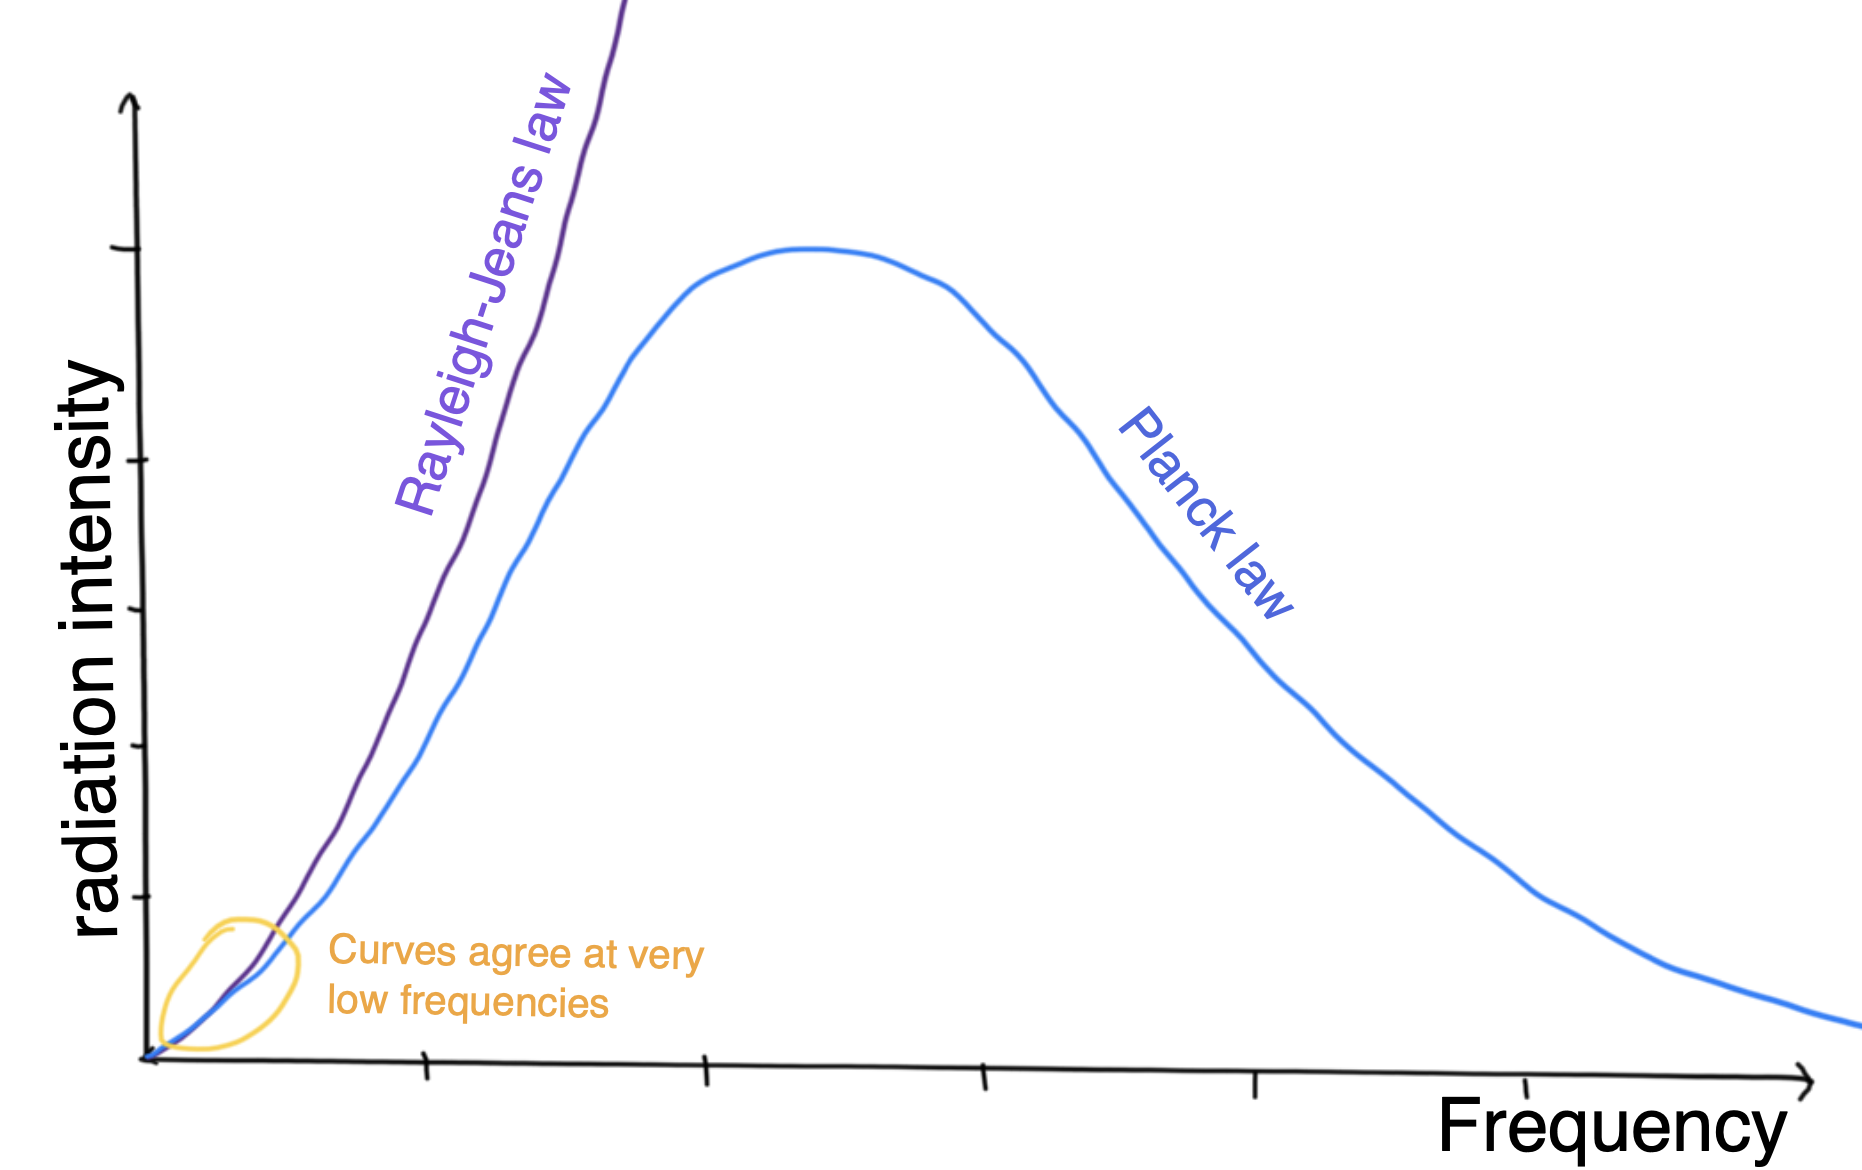
\includegraphics[scale=0.15]{qm1.png}
\end{center}

\subsection{Photoelectric effect (1905)}
\paragraph{Classical expectation}
Consider a metal surface in a vacuum, which is hit by light with angular frequency \( \omega \).
When the radiation hits the surface of the metal, electrons were emitted.
Classically, we would expect that:
\begin{enumerate}
	\item Since the incident light carries energy $ \propto $ its intensity, increasing the intensity we should have sufficient energy to break the bonds of the electrons with the atoms of the metal.
	\item Since the intensity and frequency are independent, light of any \( \omega \) would eventually cause electrons to be emitted, given a high enough intensity.
	\item The emission rate should be constant.
\end{enumerate}
\begin{center}
    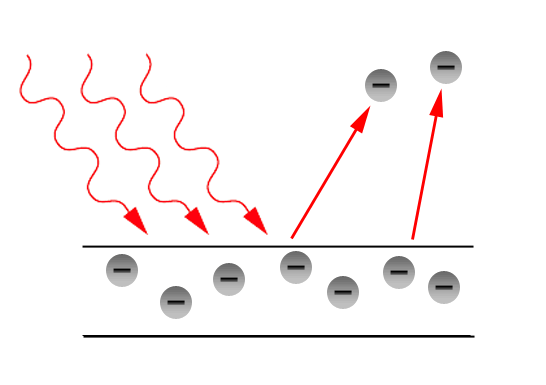
\includegraphics[scale=0.5]{qm2.png}
\end{center}
\paragraph{Inconsistency with experiment and interpretation}
Experiments showed that
\begin{enumerate}
	\item The maximum energy \( E_{\max} \) of emitted electrons depended on \( \omega \) not $I$. 
	\item Below a given threshold \( \omega_{\min} \), no electron emission.
	\item The emission rate $ \nearrow $ as $ I \nearrow $.
\end{enumerate}
Einstein's explanation for this phenomenon was that 
\begin{enumerate}
    \item The light was \textit{quantised} into small quanta, called \textbf{photons}.
    \item Each carries \( E = \hbar \omega, \mathbf{p}= \hbar \mathbf{k} \).
    \item Each photon could liberate only one electron.
    Thus,
    \[
        E_{\max} = \hbar \omega - \Phi
    \]
    where \( \Phi \) is the binding energy of the electron with the metal aka \textbf{work function}.
    \item $ \nearrow I \Leftrightarrow \nearrow \# \text{ of photons}\Leftrightarrow \nearrow \text{ scattering}\Leftrightarrow \text{higher }e^- \text{ emission rate}$.
\end{enumerate}

\subsection{Compton scattering (1923)}

X-rays were emitted towards a crystal, scattering free electrons.
The X-ray should then be deflected by some angle \( \theta \).

\begin{center}
    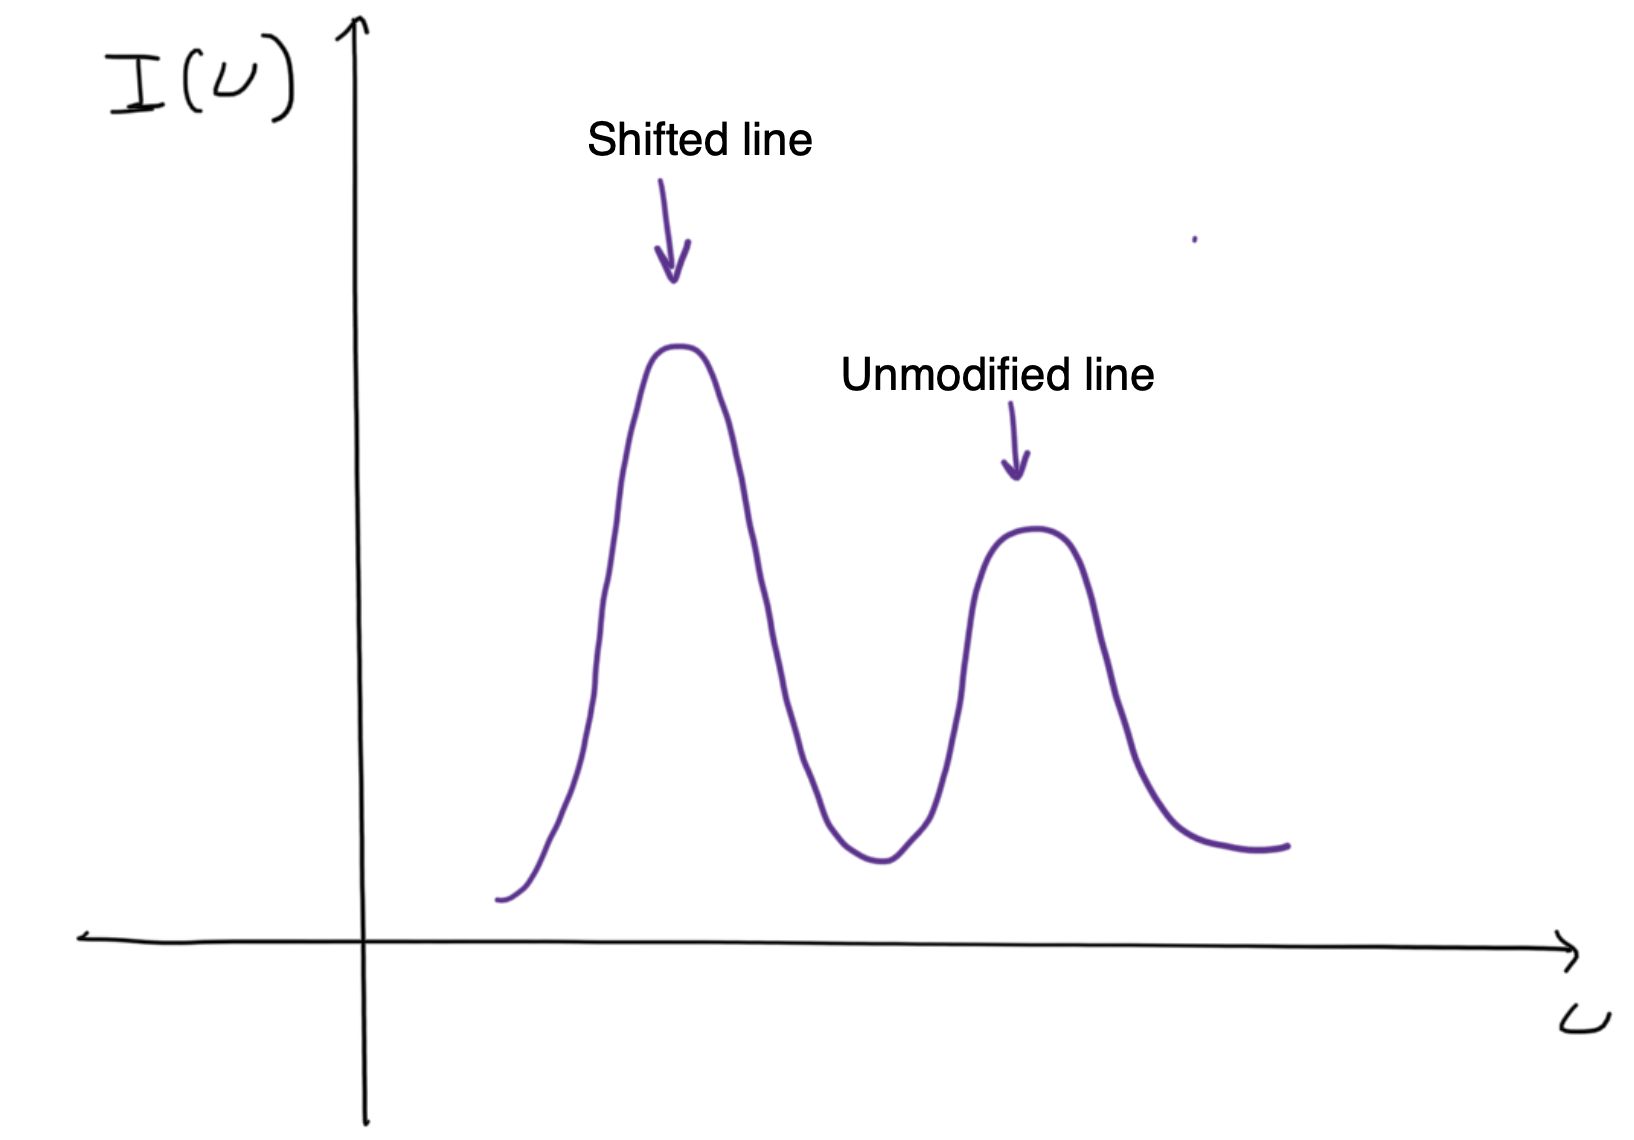
\includegraphics[width=0.5\textwidth]{qm3.png}
    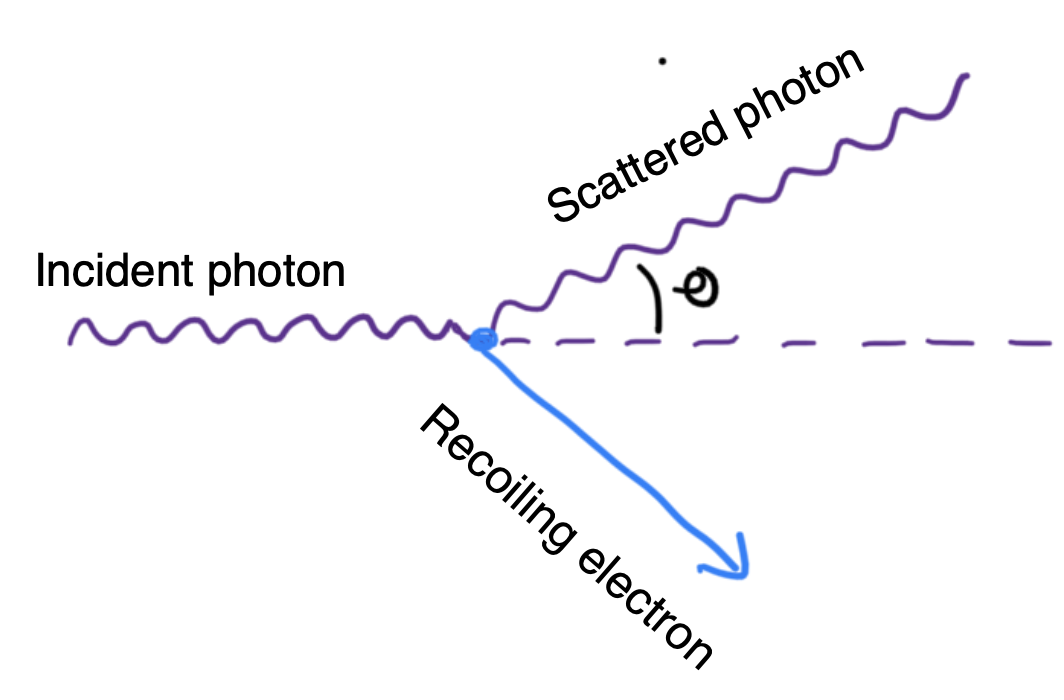
\includegraphics[width=0.45\textwidth]{qm4.png}
\end{center}

Classically, for a given \( \theta \) we would expect that the intensity as a function of \( \omega \) would have a maximum at \( \omega_0 \), the frequency of the incoming X-rays.
This is because we would not expect \( \omega \) to change much after scattering an electron.

However, there was another peak at \( \omega' \), which was dependent on the angle \( \theta \).
In fact, considering the photon and electron as a relativistic system of particles, we can derive (from IA Dynamics and Relativity),
\[
	2 \sin^2 \frac{\theta}{2} = \frac{mc}{\abs{\vb q}} - \frac{mc}{\abs{\vb p}}
\]
where \( \vb p \) is the initial momentum and \( \vb q \) is the final momentum.
Assuming \( E = \hbar \omega \) and \( \vb p = \hbar \vb k \),
\[
	\abs{\vb p} = \hbar \abs{\vb k} = \hbar \frac{\omega}{c}\quad \abs{\vb q} = \hbar \abs{\vb k'} = \hbar\frac{\omega'}{c}
\]
Hence,
\[
	\frac{1}{\omega} = \frac{1}{\omega'} + \frac{\hbar}{mc}(1-\cos\theta)
\]
So the frequency of the outgoing X-ray should have an angular frequency which is shifted from the original.
The expected peak was actually caused by X-rays simply not interacting with the electrons.

\subsection{Atomic spectra}
The Rutherford scattering experiment: shoot \( \alpha \) particles at some thin gold foil.
Most particles travelled through the foil, some were slightly deflected, and some were deflected completely back.
This indicated that the gold foil was mostly comprised of vacuum and there was a high density of positive charge within the atom. 
Which leads to Rutherford's model that electrons would orbit around the nucleus.

\begin{center}
    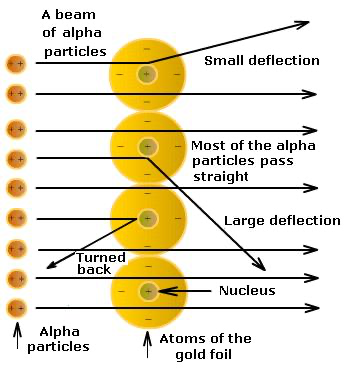
\includegraphics[width=0.5\textwidth]{qm5.png}
\end{center}

However, there were problems with this model:
\begin{enumerate}
	\item If the electrons in orbits moved, they would radiate and lose energy.
	      However if the electrons were static, they would simply collapse and fall into the nucleus.
	\item This model did not explain the atomic spectra, the observed frequencies of light absorbed or emitted by an atom when electrons change energy levels.
\end{enumerate}
The spectra had frequency
\[
	\omega_{mn} = 2 \pi c R_0 \qty(\frac{1}{n^2} - \frac{1}{mc}); \quad m, n \in \mathbb N, m > n
\]
where \( R_0 \) is the Rydberg constant, approximately \( \SI{1e7}{\per\metre} \).

In 1913 Niels Bohr observed that these problems could be resolved in a way consistent with Planck's and Einstein's earlier postulates, if we suppose that the electron orbits of hydrogen atoms are quantised so that the orbital angular momentum takes one of a discrete set of values
\[
L=n \hbar \quad \text { with } \quad n \in \mathbb{N}, n>0 .
\]
\begin{proposition}
    Quantisation of $L \implies $ quantisation of $r,v,E$. 
\end{proposition}
\begin{proof}
    In a circular motion, the angular momentum is given by
\[
L=m_e v r,
\]
we can derive
\[
v \equiv v_n=\frac{n \hbar}{m_e r} .
\]
Coulomn force 
\[
    F_{\text {Coulomb }}=\frac{e^2}{4 \pi \epsilon_0} \frac{1}{r^2}=m_e \frac{v^2}{r} 
\]
So 
\[
    r \equiv r_n=n^2\left(\frac{4 \pi \epsilon_0}{m_e e^2} \hbar^2\right) \equiv n^2 r_0, \quad
        r_0=\frac{4 \pi \epsilon_0 \hbar^2}{m_e e^2} \sim \SI{0.53e-10}{\metre}
\]
$a_0$ is the \textbf{Bohr radius}. Energy is also quantised: 
\[
    E_n=\frac{1}{2} m_e v_n^2-\frac{e^2}{4 \pi \epsilon_0} \frac{1}{r_n}=-\frac{e^2}{8 \pi \epsilon_0 a_0} \frac{1}{n^2}=-\frac{e^4 m_e}{32 \pi^2 \epsilon_0^2 \hbar^2} \frac{1}{n^2} \equiv \frac{E_1}{n^2}
\]
where $ E_1=-\left(e^4 m_e\right) /\left(32 \pi^2 \epsilon_0^2 \hbar^2\right) \sim \SI{-13.6}{eV} $ is the \textbf{groud level}. 
\end{proof}

\begin{center}
    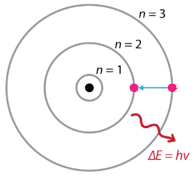
\includegraphics[scale=0.5]{qm6.png}
\end{center}

Note that 
\[
R_0=\frac{m_e c}{2 \hbar}\left(\frac{e^2}{4 \pi \epsilon_0 \hbar c}\right)^2
\]
agrees well with the experimentally determined values of the Rydberg constant.

\subsection{Wave-like behaviour of particles (1923)}
De Broglie hypothesised that any particle of any mass is associated with a wave with
\[
	\omega = \frac{E}{\hbar}; \quad \vb k = \frac{\vb p}{\hbar}
\]
This hypothesis made sense of the quantisation of electron angular momentum; if the electron lies on a circular orbit then \( 2 \pi r = n \lambda \) where \( \lambda \) is the wavelength of the electron.
However,
\[
	p = \hbar k = \hbar \frac{2 \pi}{\lambda} \implies L = m_e v r = p r = \hbar \frac{2 \pi}{\lambda} \frac{n \lambda}{2 \pi} = n \hbar
\]
Hence the angular momentum must be quantised.
The electron diffraction experiment showed that this hypothesis was true, by showing that electrons behaved sufficiently like waves.
Interference patterns were observed with \( \lambda = \frac{2 \pi}{\abs{\vb k}} = \frac{2 \pi k}{\abs{\vb p}} \) compatible with the De Broglie hypothesis.

\clearpage

\part{Foundations of Quantum Mechanics}
\section{Wavefunctions and probabilistic interpretation}
\subsection{Probabilistic interpretation}

In classical mechanics, a particle is described with \( \vb x, \dot{\vb x} \) or \( \vb p = m \dot{\vb x} \).
In quantum mechanics, it is described by a state \( \psi= \psi(\vb x, t) \) called the wavefunction.

\begin{definition}
    A wavefunction is a function \( \psi(\vb x, t) \colon \mathbb R^3 \to \mathbb C \) that satisfies certain mathematical properties dictated by its physical interpretation.
\end{definition}
\begin{note}
    \( t \) is considered a fixed external parameter, so it is not included in the function's type.
\end{note}

\paragraph{The physical interpretation} is called \textbf{Born's rule.}

\begin{proposition}[Born's rule]
    The probability density for a particle to be at some point \( \vb x \) at \( t \) is given by 
    \[
        \rho(\mathbf{x},t) \propto \left| \psi(\mathbf{x},t) \right| ^2. 
    \]
    The probability that the particle lies in some small volume \( V \) centred at \( \vb x \) is given by 
    \[
        \rho(\vb x, t) \dd{V}.
    \]
\end{proposition}

\paragraph{The mathematical properties} Now we can list the properties explicitly:
\begin{enumerate}
    \item The particle must be somewhere, so the wave function must be \textit{normalisable}, or \textit{square-integrable} in \( \mathbb R^3 \):
    \[
        \int_{\mathbb R^3} \psi^*(\vb x, t) \psi(\vb x, t) \dd{V} = \int_{\mathbb R^3} \abs{\psi(\vb x, t)}^2 \dd{V} = N \in (0, \infty).
    \]
    \item Total probability is 1, which leads to normalised wavefunction
    \[
        \overline{\psi}(\vb x, t) = \frac{1}{\sqrt{N}} \psi(\vb x, t) \iff \int_{\mathbb R^3} \abs{\overline{\psi}(\vb x, t)}^2 \dd{V} = 1.
    \]
    Hence, \( \rho(\vb x,t) = \abs{\overline{\psi}(\vb x,t)}^2 \).
\end{enumerate}

\begin{note}
    \begin{enumerate}
        \item Often we drop the bar and just write wavefunction as $ \psi $, and normalise at the end. 
        \item If $ \widetilde{\psi}(\mathbf{x},t) = e^{i\alpha} \psi(\mathbf{x},t) $ with $ \alpha\in \mathbb{R} $, then $ \left| \widetilde{\psi}(\mathbf{x},t) \right|^2 = \left| \psi(\mathbf{x},t) \right| ^2  $, i.e. $ \psi,\widetilde{\psi} $ are \textit{equivalent states}. 
        \item *We can think of states as arrays in the vector space of wavefunctions.
        We can then describe the equivalence class \( [\psi] \) as the set of all functions \( \phi \) such that \( \phi = \lambda \psi \), for some \( \lambda \in \mathbb C \setminus \qty{0} \), since we must retain the condition that \( \phi \) is normalisable.
    \end{enumerate}
\end{note}

\paragraph{Compare linear algebra to QM} Linear algebra and quantum mechancis have a lot of similarities: 
\begin{center}
\begin{tabular}{cc}
    \toprule 
    \textbf{Linear Algebra} & \textbf{Quantum Mechanics} \\ \midrule
    Vector: $\displaystyle \mathbf{v} = (v_1,\dots,v_n)$ & State $ \psi: \mathbf{x} \mapsto \psi(\mathbf{x},t) $ \\[0.4em] 
    Vector space: $ \mathbb{C}^n $ & Hilbert space: $ L^2( \mathbb{R}^{3}) $ \\[0.4em]  
    Inner product: $ (\mathbf{v},\mathbf{w}) = \mathbf{v}^\dagger \mathbf{w} $ & Inner product: $\displaystyle (\psi,\phi) = \int_{\mathbb{R}^3} \psi^*(\mathbf{x},t)\phi(\mathbf{x},t) \,\mathrm{d}V$ \\[1em]  
    Matrix: $ T = (T_{ij}) $ & Operators: $ \hat{O}: L^2( \mathbb{R}^{3})\to L^2( \mathbb{R}^{3}) $\\
    \bottomrule
\end{tabular}
\end{center}

\subsection{Hilbert space}
The set of all states forms a space, called Hilbert space. 
\begin{definition}
    The set of all square integrable functions in $ \mathbb{R}^3 $ is called \textbf{Hilbert space}, denoted as $ \mathcal{H} \equiv L^2(\mathbb{R}^3) $.
\end{definition}
Check that it is a vector space: 
\begin{proposition}
    $ \mathcal{H} $ is a vector space. Since $ \mathcal{H} \subseteq \mathbb{C}^{\mathbb{R}^3} $, this is equivalent to $ \psi_1,\psi_2\in \mathcal{H} \implies a_1 \psi_1+a_2\psi_2\in \mathcal{H} $, where $ a_1,a_2\in \mathbb{C} $.
\end{proposition}

\begin{proof}
    It suffices to show that: if $\psi_1(\mathbf{x}, t)$ and $\psi_2(\mathbf{x}, t)$ are both normalisable,
    \[
    \int_{\mathbb{R}^3}\left|\psi_1(\mathbf{x}, t)\right|^2 d V=N_1<\infty, \quad \int_{\mathbb{R}^3}\left|\psi_2(\mathbf{x}, t)\right|^2 d V=N_2<\infty,
    \]
    then their linear combination is also normalisable.

    For any two complex number $z_1$ and $z_2$, the triangle inequality states that
    \[
    \left|z_1+z_2\right| \leq\left|z_1\right|+\left|z_2\right|,
    \]
    and
    \[
    \left(\left|z_1\right|-\left|z_2\right|\right)^2 \geq 0 \Rightarrow 2\left|z_1\right|\left|z_2\right| \leq\left|z_1\right|^2+\left|z_2\right|^2 .
    \]
    If we apply these relations for $z_1=a_1 \psi_1$ and $z_2=a_2 \psi_2$, we get
    \begin{align*}
        \int_{\mathbb{R}^3}|\psi(&\mathbf{x}, t)|^2 \dd V =\int_{\mathbb{R}^3}\left|a_1 \psi_1(\mathbf{x}, t)+a_2 \psi_2(\mathbf{x}, t)\right|^2 \dd V \\
        & \leq \int_{\mathbb{R}^3}\left(\left|a_1 \psi_1(\mathbf{x}, t)\right|+\left|a_2 \psi_2(\mathbf{x}, t)\right|\right)^2 \dd V \\
        &=\int_{\mathbb{R}^3}\left(\left|a_1 \psi_1(\mathbf{x}, t)\right|^2+\left|a_2 \psi_2(\mathbf{x}, t)\right|^2+2\left|a_1 \psi_1(\mathbf{x}, t)\right|\left|a_2 \psi_2(\mathbf{x}, t)\right|\right) \dd V \\
        & \leq \int_{\mathbb{R}^3}\left(2\left|a_1 \psi_1(\mathbf{x}, t)\right|^2+2\left|a_2 \psi_2(\mathbf{x}, t)\right|^2\right) \dd V \\
        &=2\left|a_1\right|^2 N_1+2\left|a_2\right|^2 N_2<\infty .\qedhere
    \end{align*}
\end{proof}

\begin{corollary}[Superposition principle]
    If $\psi_1$ and $\psi_2$ correspond to allowed states of a system, then so does the state $\psi$, where
    \[
    \psi=a_1 \psi_1+a_2 \psi_2 \neq 0
    \]
    for arbitrary complex numbers $a_1$ and $a_2$. 
\end{corollary}
This is known as the \textbf{superposition principle}.

\subsection{Inner product}
We can naturally define an inner product on this vector space, in analogy with the finite-dimensional case.

\begin{definition}
    The inner product of two wavefunctions $\psi(\mathbf{x}, t)$ and $\phi(\mathbf{x}, t)$ at a time $t$ is given by
    \[
    (\psi, \phi) \equiv \int_{\mathbb{R}^3} \psi^*(\mathbf{x}, t) \phi(\mathbf{x}, t) \dd V .
    \]
\end{definition}

\begin{theorem}
    The following statements hold.
\begin{enumerate}[(i)]
	\item \( (\psi, \phi) \) exists for all \( (\psi, \phi) \in \mathcal H \)
	\item \( (\psi, \phi^*) = (\phi, \psi) \)
	\item The inner product is antilinear in the first entry, and linear in the second entry
	\item Tor continuous \( \psi \), \( (\psi, \psi) = 0 \) if and only if \( \psi=0 \).
\end{enumerate}
\end{theorem}
\begin{proof}
    (ii)-(iv) are from definition, so we only prove (i). 

    Take $\psi(\mathbf{x}, t)$ and $\phi(\mathbf{x}, t)$. By Cauchy-Schwartz inequality,
    \[
    \left|\int_{\mathbb{R}^3} \psi^*(\mathbf{x}, t) \phi(\mathbf{x}, t) \dd V\right| \leq \sqrt{\int_{\mathbb{R}^3}|\psi(\mathbf{x}, t)|^2 \dd V \int_{\mathbb{R}^3}|\phi(\mathbf{x}, t)|^2 \dd V} .
    \]
    So if both terms on RHS are finite, then also the inner product is finite.
\end{proof}

Using the definition of inner product, we can define (or redefine) a series of important properties of wavefunctions:

\begin{definition}
    \begin{enumerate}
        \item The \textbf{norm} of a wavefunction is $\|\psi\|=\sqrt{(\psi, \psi)}$.
        \item A wavefunction $\psi$ is \textbf{normalised} if $\|\psi\|=1$.
        \item Two wavefunctions $\psi, \phi$ are \textbf{orthogonal} if $(\psi, \phi)=0$.
        \item A set of wavefunctions $\left\{\psi_n\right\}$ is \textbf{orthonormal} is they are normalised and mutually orthogonal:
        \[
        \left(\psi_m, \psi_n\right)=\delta_{m n} .
        \]
        \item A set of wavefunctions $\left\{\psi_n\right\}$ is \textbf{complete} if any other wavefunction in Hilbert space can be expressed as a linear combination of them:
        \[
        \phi=\sum_{n=0}^{\infty} c_n \psi_n
        \]
    \end{enumerate}
\end{definition}

\begin{lemma}
    If the wavefunctions $\left\{\psi_n\right\}$ that form a complete set are also an orthonormal set, the coefficients of $ \phi $ in $ \{\psi_n\} $ are given by:
    \[
    c_n=\left(\psi_n, \phi\right).
    \]
\end{lemma}
\begin{proof}
    \begin{align*}
        \left(\psi_n, \phi\right) &=\left(\psi_n, \sum_{m=0}^{\infty} c_m \psi_m\right) \\
        &=\sum_{m=0}^{\infty} c_m\left(\psi_n, \psi_m\right)=\sum_{m=0}^{\infty} c_m \delta_{m n}=c_n.\qedhere
    \end{align*}
\end{proof}

\section{Time-dependent Schr\"odinger equation (TDSE)}
\subsection{Definition of TDSE}\
\vspace{-1.5em}
\begin{definition}
	The evolution of the wavefunction over time is given by the \textbf{time-dependent Schr\"odinger equation (TDSE)},
	\[
		i\hbar \pdv{\psi}{t} = -\frac{\hbar^2}{2m} \laplacian \psi + U \psi
	\]
	where \( U = U(x) \) is a real potential energy term.
\end{definition}

\begin{remark}
	This equation is a first-order differential equation in \( t \).
	Contrast this to Newton's second law, which is a second-order differential equation in \( t \).
	This implies that we only need a single initial condition \( \psi(x,t_0) \) to determine all future behaviour.
\end{remark}
\begin{remark}
	Note the asymmetry between the spatial and temporal components: there is only a first derivative in time but a second derivative in space.
	This implies that this equation is incompatible with relativity, where time and space must be treated equitably.
\end{remark}
One way to conceptualise the TDSE is by letting \( \psi \) be some wave defined by
\[
	\psi(x,t) = \exp[ i(k \cdot x - \omega t) ]
\]
Then, the De Broglie hypothesis (\( k = p/\hbar, \omega = E/m \)) implies that
\[
	\psi(x,t) = \exp\qty[\frac{i}{\hbar}\qty(p \cdot x - \frac{p^2}{2m}t)]
\]
which is a solution to the TDSE.

\subsection{Conservation of probability}\
\vspace{-1.5em}
\begin{proposition}
    Any TDSE preserves normalization of the wavefunction $\psi$. 
\end{proposition}
\begin{proof}
    We will show that (Recall Born's rule)
    \[
        \frac{\mathrm{d}}{\mathrm{d}t} \int_{\mathbb{R}^3} | \psi(\mathbf{x},t)|^2 \,\mathrm{d}V = 0 \iff \int_{\mathbb{R}^3} | \psi(\mathbf{x},t)|^2 \,\mathrm{d}V = \text{const}.
    \]
    Notice that 
    \begin{align*}
        \frac{\mathrm{d}}{\mathrm{d}t} \int_{\mathbb{R}^3} | \psi|^2 \,\mathrm{d}V &= \int_{ \mathbb{R}^{3}} \frac{\partial }{\partial t}|\psi|^2  \,\mathrm{d}V\\ 
        &=\int_{\mathbb{R}^3} \frac{\partial }{\partial t}(\psi^* \psi)  \,\mathrm{d}V\\ 
        &= \int_{\mathbb{R}^3} \psi^* \frac{\partial \psi}{\partial t} + \psi\frac{\partial \psi^*}{\partial t}   \,\mathrm{d}V. 
    \end{align*}
    By TDSE, 
    \[
        \frac{\partial \psi}{\partial t} = \frac{i\hbar}{2m}\nabla^2 \psi - \frac{i}{\hbar} U \psi,\quad \frac{\partial}{\partial t} \psi^*=-\frac{i \hbar}{2 m} \nabla^2 \psi^*+\frac{i}{\hbar} U \psi^*,
    \]
    so 
    \[
        \frac{\partial}{\partial t}|\psi|^2=\frac{i \hbar}{2 m}\left(\psi^* \nabla^2 \psi-\psi \nabla^2 \psi^*\right)=\nabla \cdot\left[\frac{i \hbar}{2 m}\left(\psi^* \nabla \psi-\psi \nabla \psi^*\right)\right]. 
    \]
    Hence the integral is 
    \begin{align*}
        \int_{ \mathbb{R}^{3}} \frac{\partial }{\partial t}|\psi|^2  \,\mathrm{d}V &= \int_{\mathbb{R}^3} \nabla \cdot\left[\frac{i \hbar}{2 m}\left(\psi^* \nabla \psi-\psi \nabla \psi^*\right)\right] \,\mathrm{d}V\\ 
        &= \int_{\partial V} \frac{i \hbar}{2 m}\left(\psi^* \nabla \psi-\psi \nabla \psi^*\right) \cdot \mathrm{d} \mathbf{S}\\ 
        &= 0 
    \end{align*}
    by divergence theorem, given that $ \psi = 0 $ on $ \partial V $, i.e. $ |\mathbf{x}|\to \infty  $. 
\end{proof}

Recall that for normalized $ \psi $,
\[
    \rho(\mathbf{x},t) = | \psi(\mathbf{x},t)|^2
\]
is the probability density function. 

\begin{proposition}[Conservation of probability]
    We have the following \textit{conservation of probability}
    \[
    \frac{\partial \rho}{\partial t}+\nabla \cdot \mathbf{j}=0,
    \]
    where
    \[
    \mathbf{j}=-\frac{i \hbar}{2 m}\left(\psi^* \nabla \psi-\psi \nabla \psi^*\right).
    \]
\end{proposition}

It is straight from the proof of the previous proposition. $ \mathbf{j} $ is called the \textbf{probability current}. 

\section{Expectation and operators}

Given the wavefunction, we would like to extract some information about the particle it represents, i.e. \textit{observe} or \textit{measure} them. 
\begin{definition}
	An \textbf{observable} is a property of the particle that can be measured.
\end{definition}

In quantum mechanics, each observable is represented by an operator acting on the state \( \psi \).

\subsection{Heuristic interpretation}
From probabilistic interpretation, each measurement is represented by an expectation value of the operator. Expecation value of an observable is the mean of infinite series of measurements performed on particles on the same state. 
\begin{example}
    The measurement on position is given by 
    \[
    \langle x \rangle  = \int_{-\infty}^{\infty} x \left| \psi(x,t) \right| ^2 \,\mathrm{d}x = \int_{-\infty}^{\infty} \psi^*(x,t) x \psi(x,t) \,\mathrm{d}x.
    \]
    Measurement on momentum is 
    \[
        \begin{aligned}
            \langle p\rangle =m \frac{\dd\langle x\rangle}{\dd t}&=m \frac{\dd}{\dd t} \int_{-\infty}^{+\infty} x|\psi(x, t)|^2 \dd x=m \int_{-\infty}^{+\infty} x \frac{\partial}{\partial t}\left(\psi^*(x, t) \psi(x, t)\right) \dd x \\
            &=\frac{i \hbar}{2} \int_{-\infty}^{+\infty} x \frac{\partial}{\partial x}\left(\psi^*(x, t) \frac{\partial \psi(x, t)}{\partial x}-\psi(x, t) \frac{\partial \psi^*(x, t)}{\partial x}\right) \dd x\\ 
            &= \int_{-\infty}^{+\infty} \psi^*(x, t)\left(-i \hbar \frac{\partial}{\partial x}\right) \psi(x, t) \dd x.
        \end{aligned}
    \]
\end{example}
In general, to calculate the expectation value of any quantity $\mathcal{Q}(x, p)$, we simply replace $p$ by $(-i \hbar \partial / \partial x)$ and insert the resulting operator between $\psi^*$ and $\psi$ and integrate over the whole space
\[
\langle\mathcal{Q}(\mathbf{x}, \mathbf{p})\rangle=\int_{\mathbb{R}^3} \psi^* \mathcal{Q}(\mathbf{x},-i \hbar \nabla) \psi \dd V
\]

\subsection{Hermitian operators}
In quantum mechanics, linear transformations are represented by linear operators $\hat{O}$, which act on wavefunctions to produce new wavefunctions of the Hilbert space $\mathcal{H}$.

\begin{definition}
	An \textbf{operator} is a linear map \(\hat{O}: \mathcal H \to \mathcal H \) such that
	\[
		\hat O(a_1 \psi_1 + a_2 \psi_2) = a_1 \hat O(\psi_1) + a_2 \hat O(\psi_2)
	\]
	where \( a_1, a_2 \in \mathbb C, \psi_1, \psi_2 \in \mathcal H \).
\end{definition}

\begin{example}
\begin{itemize}
    \item Finite differential operators
    \[
    \sum_{n=0}^N p_n(x) \frac{\partial^n}{\partial x^n}
    \]
    where the $p_n(x)$ are polynomials. in $x$. Note that this includes the $\hat{p}$ and $\hat{x}$.
    \item the translation operators
    \[
    \hat{S}_a: \quad \psi(x) \rightarrow \psi(x-a)
    \]
    \item the parity operator
    \[
    \hat P: \quad \psi(x) \rightarrow \psi(-x)
    \]
\end{itemize}
\end{example}

\begin{definition}
    The \textbf{Hermitian conjugate} $\hat{O}^{\dagger}$ of an operator $\hat{O}$ is the operator such that
    \[
    \left(\hat{O}^{\dagger} \psi_1, \psi_2\right)=\left(\psi_1, \hat{O} \psi_2\right)
    \]
    for all normalisable wavefunctions $\psi_1, \psi_2 \in \mathcal{H}$.
\end{definition}
From Vectors and Matrices, 
\begin{enumerate}
    \item $\left(a_1 \hat{A}_1+a_2 \hat{A}_2\right)^{\dagger}=a_1^* \hat{A}_1^{\dagger}+a_2^* \hat{A}_2^{\dagger}$,
    \item $(\hat{A} \hat{B})^{\dagger}=\hat{B}^{\dagger} \hat{A}^{\dagger}$.
\end{enumerate}
\begin{definition}
    An operator $ \hat{O} $ is \textbf{Hermitian} if $ \hat{O} = \hat{O}^{\dagger} $.
\end{definition}

Most of the operators we deal with are hermitian: 
\begin{example}
    \begin{itemize}
        \item position
        \[
        \hat{x}: \quad \psi(x, t) \mapsto x \psi(x, t),
        \]
        \item momentum
        \[
        \hat{p}: \quad \psi(x, t) \mapsto-i \hbar \frac{\partial \psi(x, t)}{\partial x} ,
        \]
        \item kinetic energy
        \[
        \hat{T}: \quad \psi(x, t) \mapsto \frac{\hat{p}^2}{2 m} \psi(x, t)=-\frac{\hbar^2}{2 m} \frac{\partial^2 \psi(x, t)}{\partial x^2},
        \]
        \item potential energy
        \[
        \hat{U}: \quad \psi(x, t) \mapsto U(\hat{x}) \psi(x, t)=U(x) \psi(x, t),
        \]
        \item total energy, sum of the kinetic and the potential energies
        \[
        \hat{H}: \quad \psi \mapsto-\frac{\hbar^2}{2 m} \frac{\partial^2}{\partial x^2} \psi(x, t)+U(x) \psi(x, t) .
        \]
        It is often called Hamitonian. 
    \end{itemize}
\end{example}

We will now describe several crucial properties of Hermitian operators.

\begin{theorem}\label{thm:2.6}
    \begin{enumerate}[(i)]
        \item The eigenvalues of Hermitian operators are real. 
        \item Eigenfunctions corresponding to different eigenvalues are orthogonal. 
        \item The discrete and continuous sets of eigenfunctions of any Hermitian operator together form a complete orthogonal basis of the physical wavefunctions, i.e. of the normalisable complex-valued wavefunctions $ \psi $. 
    \end{enumerate}
\end{theorem}
\begin{proof}
    See Vectors and Matrices, and Dr Ubiali's notes. 
\end{proof}

\subsection{Expectation values and operators}
Let $O$ be an observation. 
\paragraph{Postulates} 
\begin{enumerate}[(1)]
    \item $O$ is represented (mathematically) by a Hermitian operator $\hat{O}$. 
    \item Outcomes are the \textit{eigenvalues} of $\hat{O}$. 
    \item If $\hat{O}$ has a discrete set of eigenfunctions $ \psi_i $ with eigenvalues $ \lambda_i $, then $ \psi_i $ are complete and we can write our (normalized) wavefunction as 
    \[
        \psi = \sum_{i} a_i \psi_i. 
    \]
    Furthermore, $ \mathbb{P}(O = \lambda_i) = |a_i|^2 = |(\psi_i,\psi)|^2 $. 
    \item If some $\lambda$ is degenerated, i.e. $ \exists \{\psi_i\}_{i\in I} $ with the samel eigenvalue $\lambda$, then
    \[
        \mathbb{P}(O=\lambda) = \sum_{i\in I} |a_i|^2
    \]
    \item $\displaystyle \sum_i\left|a_i\right|^2=\sum_i\left(a_i \psi_i, a_i \psi_i\right)=\sum_{i, j}\left(a_i \psi_i, a_j \psi_j\right)=(\psi, \psi)=1$. 
    \item (Projection Postulate). If at time $t$, the measurement $ O=\lambda_i $, $ \psi $ immediately becomes $\psi_i$.  
    \item Degeneracy in (6): If at time $t$, $ O = \lambda $, then $ \psi = \sum_{i\in I} a_i \psi_i $. 
\end{enumerate}

\begin{definition}
    The \textbf{projection operator} given $ \psi = \sum_i a_i \psi_i = \sum_i (\psi_i,\psi)\psi_i $ is given by 
    \[
        \hat{P}_i: \psi \mapsto (\psi_i,\psi)\psi_i. 
    \]
\end{definition}

Hence the expectation is essentially summing over $ |(\psi,\psi_i)|^2 \lambda_i $: 
\[
    \sum_i\left|\left(\psi, \psi_i\right)\right|^2 \lambda_i 
        =\left(\sum_i\left(\psi, \psi_i\right) \psi_i, \sum_j \lambda_j\left(\psi, \psi_j\right) \psi_j\right)=(\psi, \hat{O} \psi)
\]
and the concept of observation (or measurement) is now formalized: 
\begin{proposition}
    The expectation of a measurement of the observable $O$ the state $\psi$ is given by 
    \[
        \langle \hat{O} \rangle_{\psi} = (\psi, \hat{O}\psi).
    \]
\end{proposition}

As usual, $ \langle \cdot \rangle_{\psi} $ is linear: 
\begin{proposition}
    $ \langle a \hat{A}+ b\hat B \rangle_{\psi} = a \langle \hat A\rangle _{\psi} + b \langle\hat B\rangle_{\psi} $, where $a,b$ are real since we are dealing with Hermitian operators.
\end{proposition}

The physics implication is that if $O$ is measured twice, the outcome of second measure (if $\Delta t$ between measures is small) is the \textit{same} as the first one with probability 1. 

\paragraph{Born's rule} If $\phi(\mathbf{x}, t)$ is the desired outcome of a measurement, then the probability of measuring such an outcome given the wavefunction $\psi(\mathbf{x}, t)$ at a time $t$ is given by
\[
|(\psi, \phi)|^2=\left|\int_{\mathbb{R}^3} \psi^*(\mathbf{x}, t) \phi(\mathbf{x}, t) \dd V\right|^2 .
\]
We say that this is the probability amplitude of $\phi$ to be found in $\psi$ at time $t$, so in a sense it measures the overlap of the two wavefunctions.

\section{Time-independent Schr\"odinger Equation (TISE)}
\subsection{Definition}
From the time-dependent version of the equation,
\[
	i\hbar \pdv{\psi}{t} = \hat H \psi
\]
we can try a solution of the form
\[
	\psi(x,t) = T(t) \chi(x)
\]
Then, we can find
\[
	i \hbar \pdv{T(t)}{t} \chi(x) = T(t) \hat H \chi(x)
\]
Then, dividing by \( T \chi \),
\[
	\frac{1}{T(t)} \qty(i \hbar \pdv{T}{t}) = \frac{\hat H \chi(x)}{\chi}
\]
Since the left and right hand sides depend only on \( x \) and \( t \) respectively but are equal, they must be equal to a separation constant \( E \in \mathbb R \).
Solving for time,
\[
	\frac{1}{T} i \hbar \pdv{T}{t} = E \implies T(t) = e^{\frac{-i Et}{\hbar}}
\]
If \( E \) were complex, \( T \) would diverge, so $T\in \mathbb{R}$.
Solving for space, we have the time-independent Schr\"odinger equation as follows.
\[
	\hat H \chi(x) = E \chi(x)
\]
Explicitly,
\begin{definition}
    The \textbf{time-independent Schr\"odinger equation} is given by 
    \[
	-\frac{\hbar^2}{2m} \laplacian{\chi(x)} + U(x) \chi(x) = E \chi(x).
\]
\end{definition}
This is an eigenvalue equation for \( \hat H \); we wish to find the eigenvalues for \( \hat H \) in the \( x \) basis.
Note that the factorised solution \( \psi = T \chi \) is just a particular class of solutions for the time-dependent Schr\"odinger equation.
However, it can be shown that any solution to the time-dependent equation can be written as a linear combination of the time-independent equation solutions.

\subsection{Stationary states}\ \vspace{-1.5em}
\begin{definition}
	With the ansatz \( \psi(x,t) = \chi(x) T(t) \), we have found a particular class of solutions of the time-independent Schr\"odinger equation:
	\[
		\psi(x,t) = \chi(x) e^{-\frac{i E t}{\hbar}}
	\]
	where \( \chi(x) \) are the eigenfunctions of \( \hat H \) with eigenvalue \( E \).
	Such solutions are called stationary states.
\end{definition}

\begin{note}
    Notice that \[
        \rho(x,t) = \abs{\psi(x,t)}^2 = \abs{\chi(x)}^2
    \]
    This explains the naming of the states as `stationary', as their probability density is independent of time.
\end{note}

By applying theorem \ref{thm:2.6} to the Hamiltonian operator we get
\begin{theorem}
    Every solution of the TDSE can be written as a superposition of stationary states $\chi(x) T(t)$.
\end{theorem}

\begin{itemize}
    \item Suppose \( E \) is quantised.
    Then, the general solution to the system is
    \[
        \psi(x,t) = \sum_{n=1}^N a_n \chi_n(x) e^{-\frac{iE_n t}{\hbar}}
    \]
    where \( N \) can be finite or infinite.
    \item In principle, we can also have a continuous energy state \( E_\alpha, \alpha \in \mathbb R \).
    We can still use the same idea:
    \[
        \psi(x,t) = \int_{\Delta \alpha} A(\alpha) \chi_\alpha(x) e^{-\frac{iE_\alpha t}{\hbar}} \dd{\alpha}
    \]
    Note that \( \abs{a_n}^2 \) and \( A(\alpha) \dd{\alpha} \) give the probability of measuring the particle energy to be \( E_n \) or \( E_\alpha \).
\end{itemize}

In general $\psi(x, t)$ is not a stationary state and thus does not have a definite energy. We can see this explicitly. Take a state $\psi$, which is the superposition of two stationary states $\psi_1$ and $\psi_2$ with two real coefficient of proportionality $a_1$ and $a_2$ and real stationary state wavefunctions $\chi_1(x)$ and $\chi_2(x)$ (for simplicity). If we compute the probability density associated to this state, we see that the it is not a constant, rather it oscillates with time. Indeed
\[
\begin{aligned}
|\psi(x, t)|^2 &=\left|a_1 \Psi_1(x, t)+a_2 \Psi_2(x, t)\right|^2 \\
&=a_1^2\left|\chi_1(x)\right|^2+a_2^2\left|\chi_2(x)\right|^2+a_1 a_2 \chi_1(x) \chi_2(x)[\exp (i \Delta E t / \hbar)+\exp (-i \Delta E t / \hbar)] \\
&=a_1^2\left|\chi_1(x)\right|^2+a_2^2\left|\chi_2(x)\right|^2+2 a_1 a_2 \chi_1(x) \chi_2(x) \cos (\Delta E t / \hbar)
\end{aligned}
\]
with $\Delta E=E_1-E_2$.
\clearpage

\part{1D Solutions of Schr\"odinger Equation}
\section{Bound states}
\subsection{Infinite potential well}
\begin{example}
    Define
\[
	U(x) = \begin{cases}
		0      & \text{for } \abs{x} \leq a \\
		\infty & \text{for } \abs{x} > a
	\end{cases}
\]

\begin{center}
    \begin{tikzpicture}
        \draw[draw=none, fill=black!20] (-4,0) rectangle (-2,3.5); 
        \draw[draw=none, fill=black!20] (2,0) rectangle (4,3.5); 
        \draw[->] (-4,0) -- (4,0); 
        \draw[->] (0,-0.5) -- (0,3);
        \draw (0,3) node[anchor=east] {$U(x)$};
        \draw (-2,0) -- (-2,3);
        \draw[dashed] (-2,3) -- (-2,3.5);
        \draw (2,0) -- (2,3);
        \draw[dashed] (2,3) -- (2,3.5);
        \draw (-2,0) node[anchor=north] {$-a$};
        \draw (2,0) node[anchor=north] {$a$};
    \end{tikzpicture}
\end{center}

For \( \abs{x} > a \), we must have \( \chi(a) = 0 \).
Otherwise, \( \chi \cdot U = \infty \).
This gives us a boundary condition, \( \chi(\pm a) = 0 \).
For \( \abs{x} \leq a \), we seek solutions of the form
\[
	-\frac{\hbar^2}{2m} \chi''(x) = E \chi(x);\quad \chi(\pm a) = 0
\]
Equivalently,
\[
	\chi''(x) + k^2 \chi(x) = 0;\quad k = \sqrt{\frac{2mE}{\hbar^2}}. 
\]
\end{example}
Since \( E > 0 \),
\[
	\chi(x) = A \sin kx + B \cos kx
\]
Imposing boundary conditions,
\[
	A \sin (k a) \pm B \cos (k a)=0 \quad \implies A \sin (k a)=0 \wedge B \cos (k a)=0
\]
Suppose \( A = 0 \), giving \( \chi(x) = B \cos kx \).
Then, imposing boundary conditions, \( \chi_n(x) = B \cos k_n x \) where \( k_n = \frac{n \pi}{2a} \), and \( n \) are odd positive integers.
These are even solutions.

Alternatively, suppose \( B = 0 \).
In this case, \( \chi(x) = A \sin kx \).
Thus, \( \chi_n(x) = A \sin k_n x \) where \( k_n = \frac{n \pi}{2a} \), and \( n \) are even nonzero positive integers.
These provide odd solutions.

We can also determine the normalisation constants by defining that the eigenfunctions of the Hamiltonian are normalised to unity.
Thus,
\[
	\int_{-a}^a \abs{\chi_n(x)}^2 = 1 \implies A = B = \sqrt{\frac{1}{a}}
\]
Hence, 
\begin{proposition}
    The general solution is given by the eigenvalues
    \[
        E_n = \frac{\hbar^2}{2n} k_n^2 = \frac{\hbar^2 \pi^2 n^2}{2ma^2}
    \]
    and eigenfunctions
    \[
        \chi_n(x) = \sqrt{\frac{1}{a}} \begin{cases}
            \cos(\frac{n \pi x}{2a}) & \text{if } n \text{ odd}  \\
            \sin(\frac{n \pi x}{2a}) & \text{if } n \text{ even}
        \end{cases}
    \]
\end{proposition}
\begin{remark}
	\begin{enumerate}
        \item Unlike classical mechanics, the ground state energy is not zero.
        \item\( \chi_n \) have \( (n+1) \) nodes in which \( \rho(x) = 0 \).
        When \( n \to \infty \), \( \rho_n(x) \) tends to a constant, which is like in classical mechanics.
        \item $\chi_n(-x)=(-1)^{n+1} \chi_n(x) .$
            This is known as \textbf{parity}.
    \end{enumerate}
\end{remark}
\begin{proposition}
	If we have a system of non-degenerate eigenstates (\( E_i \neq E_j \)),  then if \( U(x) = U(-x) \) the eigenfunctions of \( \hat H \) must be either odd or even.
\end{proposition}
\begin{proof}
	The time-independent Schr\"odinger equation is invariant under \( x \mapsto -x \) if \( U \) is even.
	Hence, if \( \chi(x) \) is a solution with eigenvalue \( E \), then \( \chi(-x) \) is also a solution.
	Since we have a non-degenerate solution, \( \chi(-x) = \chi(x) \) hence the solutions must be the same up to a normalisation factor.
	For consistency, \( \chi(x) = \chi(-(-x)) = \alpha \chi(-x) = \alpha^2 \chi(x) \).
	Hence \( \alpha = \pm 1 \), so \( \chi \) is either odd or even.
\end{proof}

\subsection{Finite potential well}

\begin{example}
    In the case of a finite potential well,
    \[
    U(x)= \begin{cases}0 & |x| \leq a \\ U_0 & |x|>a,\end{cases}
    \]
    \begin{center}
        \begin{tikzpicture}
            \draw[->] (-4,0) -- (4,0); 
            \draw[->] (0,-0.5) -- (0,3);
            \draw (0,3) node[anchor=east] {$U(x)$};
            \draw (-2,0) -- (-2,3) -- (-3.5,3) node[anchor=east] {$U_0$};
            \draw (2,0) -- (2,3) -- (3.5,3) node[anchor=west] {$U_0$};
            \draw (-2,0) node[anchor=north] {$-a$};
            \draw (2,0) node[anchor=north] {$a$};
        \end{tikzpicture}
    \end{center}
    the stationary states obey
    \[
    -\frac{\hbar^2}{2 m} \chi^{\prime \prime}(x)+U(x) \chi(x)=E \chi(x) .
    \]
\end{example}

Classically, if \( E < U_0 \), the particle has insufficient energy to escape the well.
We will only consider eigenstates with \( E < U_0 \) here, but we will find that it is possible in quantum mechanics to escape the well with positive probability.

Search for even functions only, odd functions can be solved independently.
If \( \abs{x} \leq a \),
\[
	-\frac{\hbar^2}{2m} \chi''(x) = E\chi(x)
\]
Equivalently,
\[
	\chi''(x) + k^2 \chi(x) = 0;\quad k = \sqrt{\frac{2mE}{\hbar^2}}
\]
The solution becomes
\[
	\chi(x) = A \sin kx + B \cos kx \implies \chi(x) = B \cos kx
\]
since we are only looking for even solutions.
In the region \( \abs{x} > a \),
\[
	-\frac{\hbar^2}{2m} \chi''(x) + U_0 \chi(x) = E \chi(x)
\]
giving
\[
	\chi''(x) - \tilde k^2 \chi(x) = 0;\quad \tilde k = \sqrt{\frac{2m(U_0 - E)}{\hbar^2}}
\]
This yields exponential solutions:
\[
	\chi(x) = C e^{\tilde k x} + D e^{-\tilde k x}
\]
Imposing the normalisability constraints, for \( x > a \) we have \( C = 0 \), and for \( x < -a \) we have \( D = 0 \).
Imposing even parity, \( C = D \) when nonzero.
Thus,
\[
	\chi(x) = \begin{cases}
		C e^{\tilde k x}  & x < -a         \\
		B \cos(kx)           & \abs{x} \leq a \\
		C e^{-\tilde k x} & x > a
	\end{cases}
\]
Now we must impose continuity of \( \chi(x) \) and its derivative at \( x = \pm a \).
First,
\[
	C e^{-\tilde k a} = B \cos(k a)
\]
The other gives
\[
	-\tilde k C e^{-\tilde k a} = -k B \sin(k a)
\]
From the ratio of both constraints,
\[
	k \tan (ka) = \tilde k
\]
From the definition of \( k, \tilde k \),
\[
	k^2 + \tilde k^2 = \frac{2mU_0}{\hbar^2}
\]
We will define some rescaled variables for convenience: \( \xi = ka \), \( \eta = \tilde k a \).
Rewriting,
\[
	\xi \tan \xi = \eta;\quad \xi^2 + \eta^2 = r_0^2;\quad r_0 = \frac{2mU}{\hbar}
\]
This may be solved graphically.
\begin{center}
    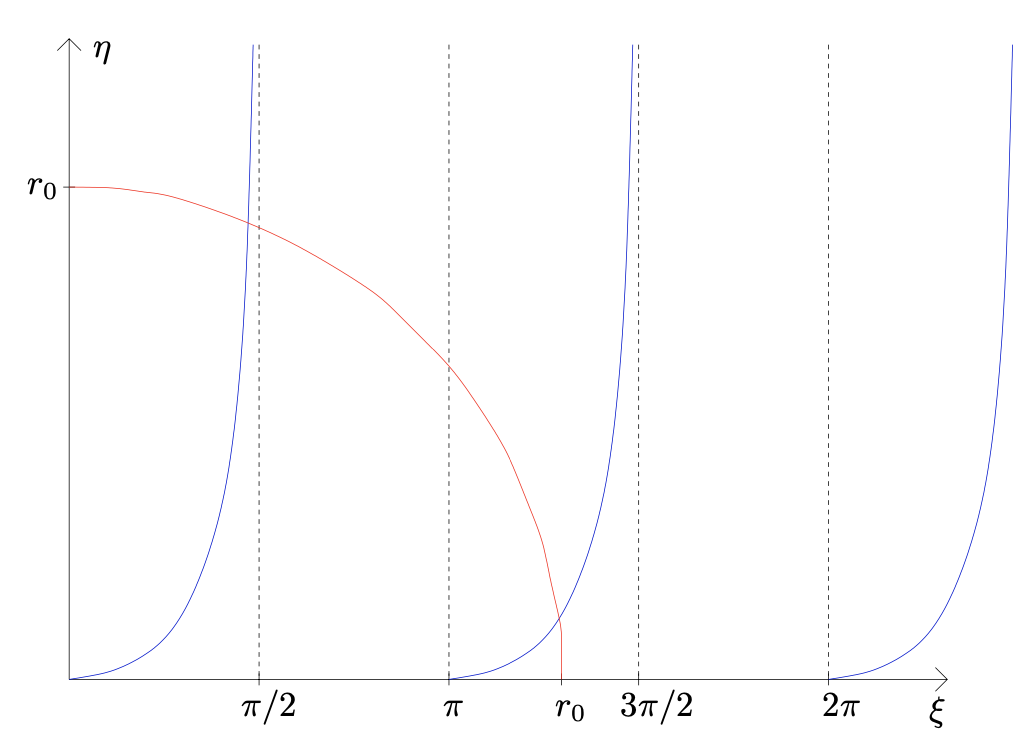
\includegraphics[scale=0.25]{qm7.png}
\end{center}
The eigenvalues of the system correspond to the points of intersection between the two equations.
There are always a finite number of possible intersections, regardless of the value of \( r_0 \).
The eigenvalues are
\[
	E_n = \frac{\hbar^2}{2 n a^2} \xi_n^2;\quad \xi \in \qty{\xi_1, \dots, \xi_n};\quad n = 1, \dots, p
\]
When \( U_0 \to \infty \), \( r_0 \to \infty \).
At this point, there are an infinite amount of intersections, so the eigenvalues of the Hamiltonian become that of the infinite well.
Further \( \chi(x) \) tends to the eigenfunctions of the infinite well.

Note that the \( \chi_n(x) \) have some positive region outside the well.
We can use the unused condition above to write \( C \) in terms of \( B \), and then we can use the normalisation condition to find \( B \).

\subsection{Harmonic oscillator}\ \vspace*{-1.5em}
\begin{example}
    Consider a parabolic potential
\[
	U(x) = \frac{1}{2} kx^2 = \frac{1}{2} m \omega^2 x^2
\]
where \( k \) is an elastic constant and \( \omega = \sqrt{\frac{k}{m}} \) is the angular frequency of the harmonic oscillator.
\end{example}
Classically, we find the solution \( x = A \cos \omega t + B \sin \omega t \).
This gives a continuous energy spectrum.
The TDSE gives
\[
	-\frac{\hbar^2}{2m} \chi''(x) + \frac{1}{2} m\omega^2 x^2 \chi(x) = E \chi(X)
\]
Since this is a bound system, we will have a discrete set of eigenvalues.
The potential is symmetric so the eigenfunctions are odd or even.
We will make the change of variables
\[
	\xi^2 = \frac{m\omega}{\hbar} x^2;\quad \varepsilon = \frac{2E}{\hbar \omega}
\]
which reformulates the TDSE as
\[
	-\dv[2]{\chi}{\xi} + \xi^2 \chi = \varepsilon \chi
\]
We will start by considering the solution for \( \varepsilon = 1 \).
In this case, \( E = \frac{\hbar \omega}{2} \) and the solution is
\[
	\chi_0(\xi) = \exp[-\frac{\xi^2}{2}]
\]
So the first eigenfunction, \( \chi_0 \), is known in terms of \( x \), given by
\[
	\chi_0(x) = A \exp[-\frac{m\omega}{2\hbar}x^2];\quad E_0 = \frac{\hbar \omega}{2}
\]
To find the other eigenfunctions, we will take the general form
\[
	\chi(\xi) = f(\xi) \exp[-\frac{\xi^2}{2}]
\]
This works because we know we have a bound solution and \( \chi \) must tend to zero quickly as \( \xi \) tends to infinity, due to the differential equation in terms of \( \xi, \varepsilon \).
To find the other eigenfunction, use variation of parameters: 
\[
    \chi(\xi) = f(\xi) e^{-\xi^2/2}
\]
Which gives
\[
	-\dv[2]{f}{\xi} + 2\xi \dv{f}{\xi} + (1-\varepsilon)f = 0
\]
Note that if \( \varepsilon = 1 \), a solution is \( f = 1 \).
We can find a power series solution to this differential equation, with \( \xi = 0 \) as a regular point.
\[
	f(\xi) = \sum_{n=0}^\infty a_n \xi^n
\]
We find
\[
	\xi \dv{f}{\xi} = \sum_{n=0}^\infty n a_n \xi^n;\quad \dv[2]{f}{\xi} = \sum_{n=0}^\infty n(n-1)a_n \xi^{n-2} = \sum_{n=0}^\infty (n+1)(n+2)a_{n+2}\xi^n
\]
Comparing coefficients of \( \xi^n \),
\[
	(n+1)(n+2) a_{n+2} - 2n a_n + (\varepsilon - 1) a_n = 0
\]
Hence,
\[
	a_{n+2} = \frac{2n - \varepsilon + 1}{(n+1)(n+2)} a_n
\]
Since the function must be either even or odd, exactly one of \( a_0 \) and \( a_1 \) must be zero.
\begin{proposition}
	If the series for \( f \) does not terminate, \( \chi \) is not normalisable.
\end{proposition}
\begin{proof}
	Suppose the series does not terminate.
	We will consider the asymptotic behaviour as \( n \to \infty \).
	\[
		\frac{a_{n+2}}{a_n} \to \frac{2}{n}
	\]
	But this is the same asymptotic behaviour as the function \( g(\xi) \) given by
	\[
		g(\xi) = \exp[\xi^2] = \sum_{m=0}^\infty \frac{\xi^{2m}}{m!} = \sum_{n=0}^\infty b_n \xi^n
	\]
	with
	\[
		b_n = \begin{cases}
			\frac{1}{m!} & n = 2m     \\
			0            & n = 2m + 1
		\end{cases}
	\]
	So asymptotically,
	\[
		\frac{b_{n+2}}{b_n} = \frac{\qty(\frac{n}{2})!}{\qty(\frac{n}{2} + 1)!} = \frac{2}{n+2} \to \frac{2}{n}
	\]
	Hence \( \chi \) would have a form asymptotically equal to
	\[
		\chi(\xi) \sim \exp[\frac{\xi^2}{2}]
	\]
	Hence \( \chi(\xi) \) would be not normalisable.
\end{proof}
Hence \( f \) must be a polynomial.
So there exists \( N \) such that \( a_{N+2} = 0 \) and \( a_N \neq 0 \).
So for this value,
\[
	2N - \varepsilon + 1 = 0 \implies \varepsilon = 2N + 1
\]
By the definition of \( \varepsilon \),
\[
	E_N = \qty(N + \frac{1}{2}) \hbar \omega
\]
In particular, \( E_{N+1} - E_N = \hbar \omega \).
The eigenfunctions are
\[
	\chi_N(\xi) = f_N(\xi) \exp[-\frac{\xi^2}{2}]
\]
with the property that
\[
	\chi_N(-\xi) = (-1)^N \chi_N(\xi)
\]
\begin{align*}
	f_0(\xi) & = 1                      \\
	f_1(\xi) & = \xi                    \\
	f_2(\xi) & = 1 - 2 \xi^2            \\
	f_3(\xi) & = \xi - \frac{2}{3}\xi^3 \\
	         & \vdots
\end{align*}

In fact one can derive a general expression (Hermite polynomials):
\[
f_n(\xi)=(-1)^n e^{\xi^2} \frac{\rmd^n}{\rmd \xi^n} e^{-\xi^2}
\]

\section{Free particles and Gaussian wavepacket}
\subsection{Free particles}\ \vspace{-1.5em}

\begin{definition}
    A free particle solution corresponds to a solution of the TISE with $U(x) \equiv 0$.
\end{definition}

The time-independent Schr\"odinger equation is
\[
	-\frac{\hbar}{2m} \chi''(x) = E\chi(x)
\]
This has solutions
\[
	\chi_k(x) = A e^{i k x},\quad k = \sqrt{\frac{2mE}{\hbar^2}}
\]
The complete solution, adding \( T(t) \), is thus
\[
	\psi_k(x,t) = \chi_k(x) e^{-i E_k t / \hbar} = A e^{i\qty(kx - \frac{\hbar k^2}{2m} t)}
\]
which are called De Broglie plane waves.
This is not a solution since
\[
	\int_{-\infty}^\infty \abs{\phi_k(x,t)} \dd{x} = \abs{A}^2 \int_{-\infty}^\infty 1 \dd{x}
\]
which diverges.

In general, any non-bound solution is non-normalisable.
This is true since \[
    \int_{-\infty}^\infty \abs{\chi(x)}^2 \dd{x} < \infty \implies \lim_{R \to \infty} \int_{\abs{x} > R} \abs{\chi(x)} \dd{x} = 0
\]
So, to solve the free particle system, we will build a linear combination of plane waves \( \chi \) to yield a normalisable solution.
This is called the \textbf{Gaussian wavepacket}.

Alternatively, we can simply ignore the problem of normalisability, and change the interpretation of \( \chi_n(x) \).

\subsection{Gaussian wavepacket}
Due to the superposition principle, we can take a continuous linear combination of the \( \psi_k \) functions.
\[
	\psi(x,t) = \int_0^\infty A(k) \psi_k(x,t) \dd{k}
\]
We can construct a suitable \( A(k) \) such that \( \psi \) is normalisable.
Choosing
\[
	A(k) = A_{\text{GP}}(k) = \exp[-\frac{\sigma}{2}(k-k_0)^2],\quad k_0 \in \mathbb R, \sigma \in \mathbb R^+
\]
produces a solution called the Gaussian wavepacket.

\begin{center}
    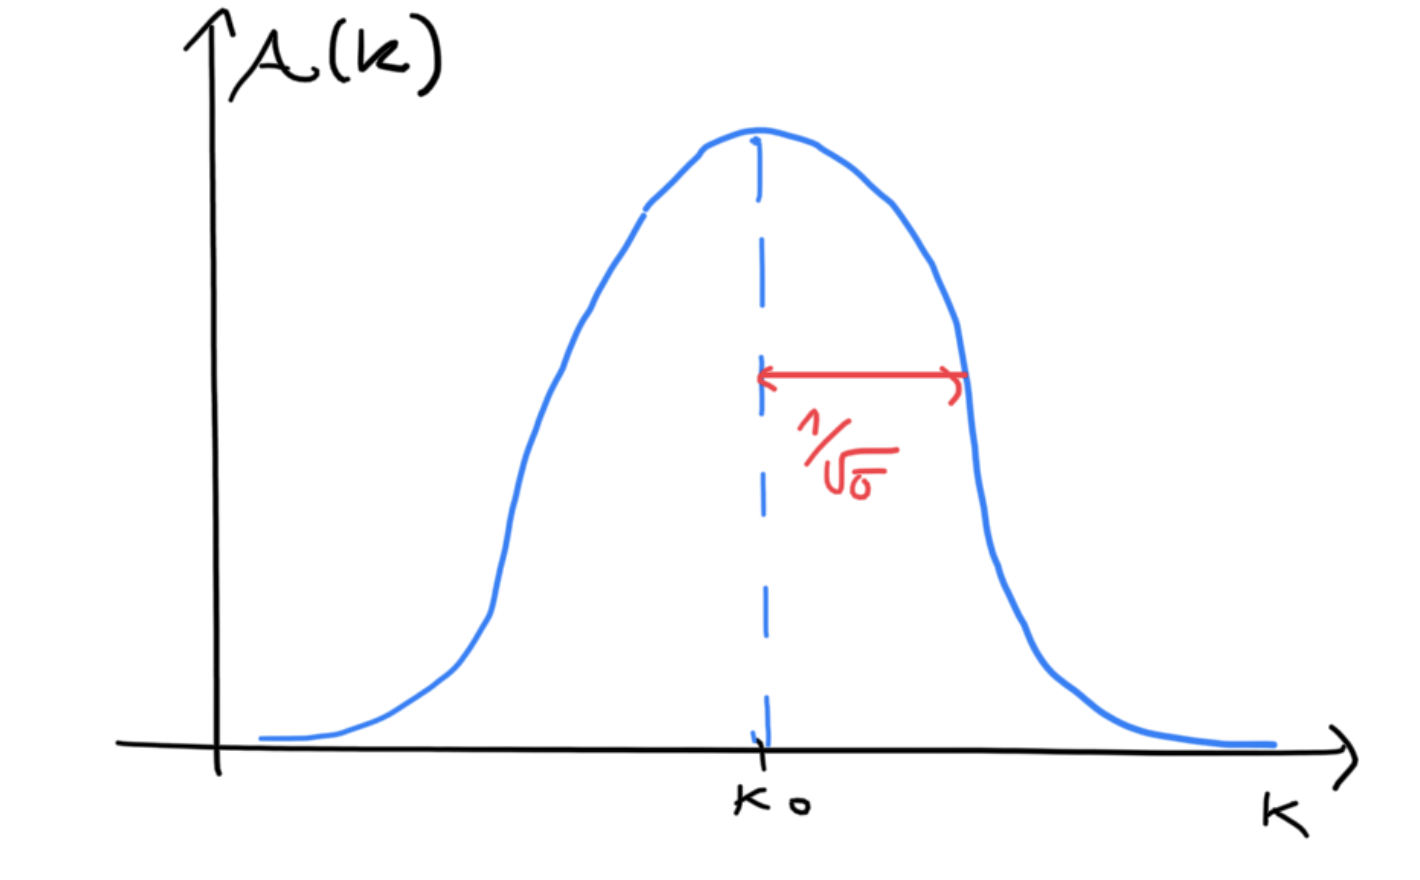
\includegraphics[scale=0.2]{qm8.png}
\end{center}

Substituting into the above,
\begin{align*}
    &\psi_{\text{GP}}(x,t) = \int_0^\infty \exp[-\frac{\sigma}{2}(k-k_0)^2] \psi_k(x,t) \dd{k} = \int_0^\infty \exp[F(k)] \dd{k}\\ 
    & F(k) = -\frac{\sigma}{2}(k-k_0)^2 + ikx - i \frac{\hbar k^2}{2m} t
\end{align*}
Can rewrite this as
\[
	F(k) = -\frac{1}{2}\qty(\sigma + \frac{i \hbar t}{m}) k^2 + (k_0 \sigma + ix)k - \frac{\sigma}{2} k_0^2
\]
We define further
\[
	\alpha \equiv \sigma + \frac{i \hbar t}{m},\quad \beta = k_0 \sigma + ix,\quad \delta = -\frac{\sigma}{2} k_0^2
\]
Completing the square,
\[
	F(k) = -\frac{\alpha}{2} \qty(k - \frac{\beta}{\alpha})^2 + \frac{\beta^2}{2\alpha} + \delta
\]
We arrive at the solution
\[
	\psi_{\text{GP}}(x,t) = \exp[\frac{\beta^2}{2\alpha} + \delta] \int_{-\infty}^\infty \exp[-\frac{\alpha}{2}\qty(k - \frac{\beta}{\alpha})^2 ] \dd{k}
\]
Under a change of variables \( \widetilde k = k - \frac{\beta}{\alpha}, u = \Im(\frac{\beta}{\alpha}) \),
\[
	\psi_{\text{GP}}(x,t) = \exp[\frac{\beta^2}{2\alpha} + \delta] \int_{\infty - iu}^{\infty - iu} \exp[-\frac{\alpha}{2} \widetilde k] \dd{\widetilde k}
\]
We arrive at the usual Gaussian integral:
\[
	I(a) = \int_{-\infty}^\infty \exp[-a x^2] \dd{x} = \sqrt{\frac{\pi}{2}}
\]
giving
\[
	\psi_{\text{GP}}(x,t) = \sqrt{\frac{2 \pi}{\alpha}} \exp[\frac{\beta^2}{2\alpha} + \delta] = \sqrt{\frac{2\pi}{\alpha}} \exp[-\frac{\sigma}{2} \frac{\qty(x - \frac{\hbar k_0}{m} t)^2}{\qty(\sigma^2 + \frac{\hbar^2 t^2}{m^2} )} ]
\]
We define \( \overline \psi_{\text{GP}} \) to be the normalised Gaussian wavefunction, so \( \overline \psi_{\text{GP}} = C \psi_{\text{GP}} \).
We can find that
\[
	\rho_{\text{GP}}(x,t) = \abs{\overline \psi_{\text{GP}}(x,t)}^2 = \sqrt{\frac{\sigma}{\pi \qty(\sigma^2 + \frac{\hbar^2 t^2}{m^2})}} \exp[ - \frac{\sigma\qty(x - \frac{\hbar k_0}{m} t)^2}{\sigma^2 + \frac{\hbar^2 t^2}{m^2}} ]
\]
This is a wavefunction whoes probability density distribution resembles a Gaussian \( e^{-x^2} \) term, with a maximum point at
\[
	\inner{x} = \int_{-\infty}^\infty \psi_{\text{GP}}^* x \psi_{\text{GP}} \dd{x} = \int_{-\infty}^\infty x \rho_{\text{GP}} \dd{x} = \frac{\hbar k_0}{m} t
\]
and a width of
\[
	\Delta x = \sqrt{\inner{x^2} - \inner{x}^2} = \sqrt{\frac{1}{2} \qty(\sigma + \frac{\hbar^2 t^2}{m^2 \sigma})}
\]
\begin{center}
    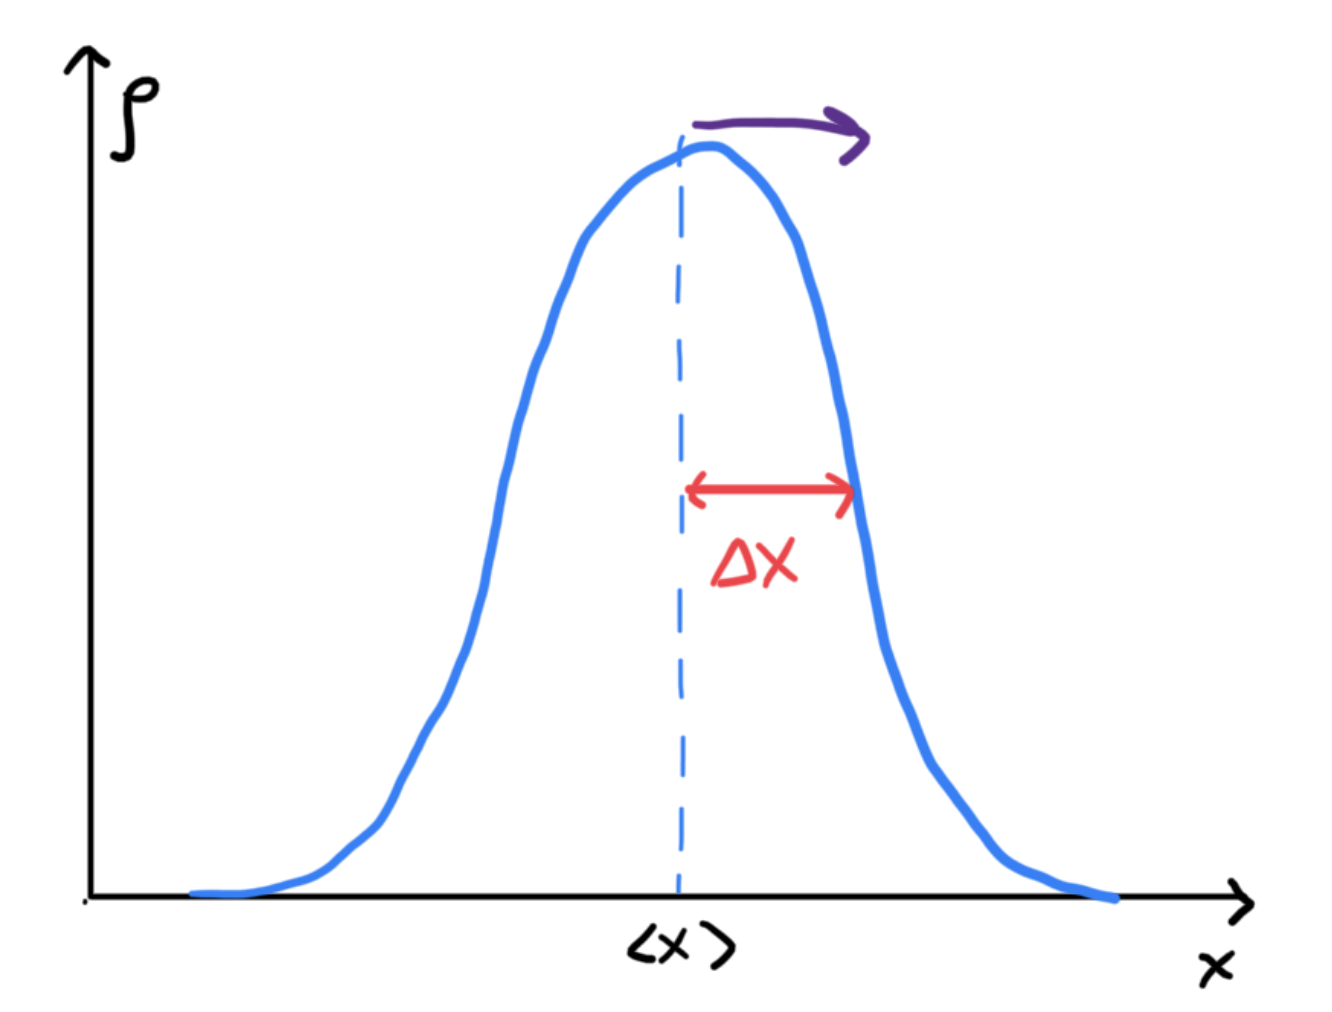
\includegraphics[scale=0.15]{qm9.png}
\end{center}

The physical interpretation is that the uncertainty of the particle's position grows with time.
In this case, we can find
\[
	\inner{p} = \int_{-\infty}^\infty -\psi_{\text{GP}}^* i \hbar \pdv{x} \psi_{\text{GP}} \dd{x} = \hbar k_0
\]
which is constant.
The uncertainty in the momentum can be found to be
\[
	\Delta p=\sqrt{\frac{\hbar^2}{2 \sigma}}
\]
Thus at $t=0$, 
\[
	\Delta x \Delta p = \frac{\hbar}{2}
\]
while $\Delta x \Delta p>\hbar / 2$ for $t>0$.
We can find for a single plane wave that
\[
	\Delta x = \infty,\quad \Delta p = 0
\]
The Gaussian wavepacket is the state with minimum uncertainty.

\subsection{Beam interpretation}

Ignore the normalisation problem and take the plane waves as the eigenfunctions of the Hamiltonian:
\[
	\chi_k(x) = Ae^{ikx},\quad \psi_k(x,t) = Ae^{ikx}e^{-\frac{i \hbar^2 k^2}{2m} t}
\]
Instead of \( \chi_k(x) \) describing a single particle, we can interpret it as a \textit{beam} of particles with momentum \( p = \hbar k \) and \( E = \frac{\hbar^2 k^2}{2m} \) with probability density
\[
	\rho_k(x) = \abs{\chi_k(x) e^{-\frac{i\hbar^2 k^2}{2m}t}}^2 = \abs{A}^2
\]
which here is interpreted as a constant average density of particles.
The probability current is given by
\[
	J_k(x,t) = - \frac{i\hbar}{2m} \qty(\psi^*_k \pdv{\psi_k}{x} - \psi_k \pdv{\psi_k^*}{x}) = -\frac{i\hbar}{2m} \abs{A}^2 2ik = \abs{A}^2 \frac{\hbar k}{m} = \abs{A}^2 \underbrace{\frac{p}{m}}_{\mathclap{\text{velocity}}}
\]
This is interpreted as the \textit{average flux} of particles.

\section{Scattering states}
We wish to investigate what happens when a particle, or beam of particles, is thrown onto a potential \( U(x) \).
In this case, suppose we have a step function
\[
	U(x) = \begin{cases} U_0 & \text{if } 0 \leq x < a \\
              0   & \text{otherwise}\end{cases}
\]
and a Gaussian wavepacket which is centred at \( x_0 \ll 0 \) moving in the \( +x \) direction, towards the spike in potential.
As \( t \gg 0 \), we end up with a probability density given by two wavepackets; one will be moving left from the spike and one will have cleared the spike and continues moving to the right.
\begin{center}
    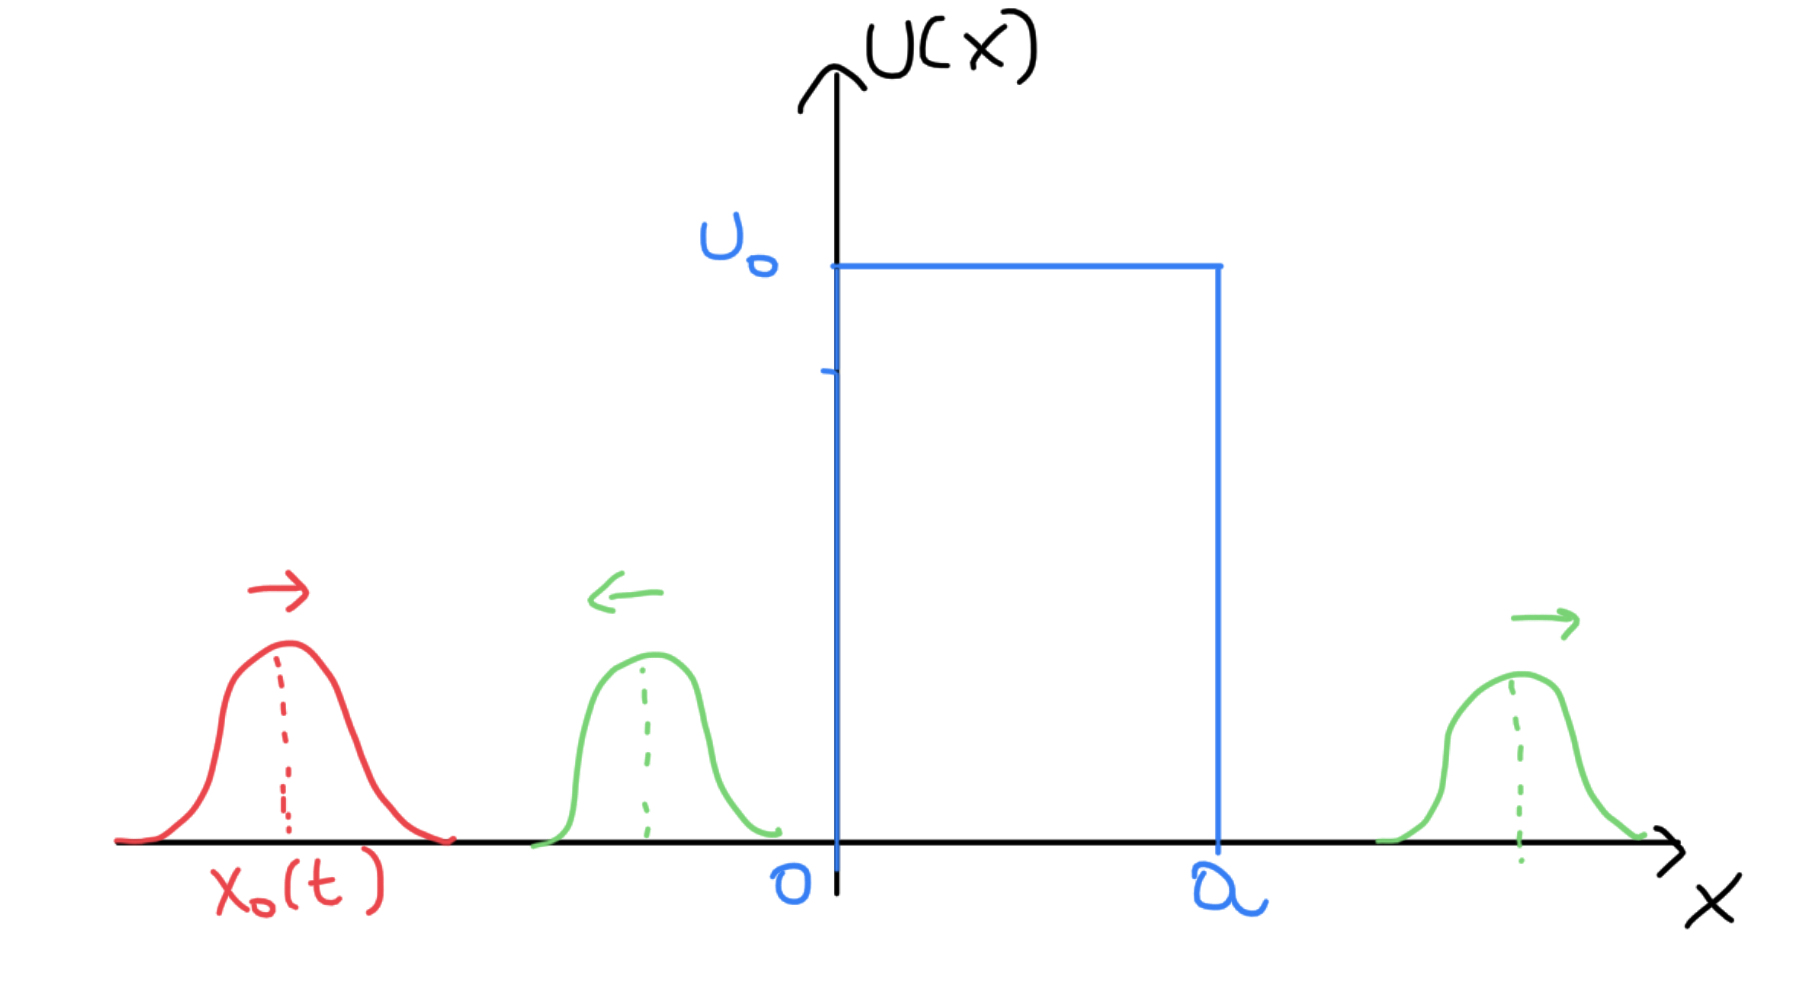
\includegraphics[scale=0.17]{qm10.png}
\end{center}
\begin{definition}
	The reflection coefficient \( R \) is
	\[
		R = \lim_{t \to \infty} \int_{-\infty}^0 \abs{\psi_{\text{GP}}(x,t)}^2 \dd{x}
	\]
	which is the probability for the particle to be reflected.
	The transmission coefficient is
	\[
		T = \lim_{t \to \infty} \int_0^\infty \abs{\psi_{\text{GP}}(x,t)}^2 \dd{x}
	\]
	By definition, \( R + T = 1 \).
\end{definition}
In practice, working with Gaussian packets is mathematically challenging (but not impossible).
The beam interpretation, by allowing us to use non-normalisable stationary state wavefunctions, greatly simplifies the computation.

\subsection{Scattering off potential step}\ \vspace{-1.5em}
\begin{example}
    Consider a potential
\[
	U(x) =
	\begin{cases}
		0   & \text{if } x \leq 0 \\
		U_0 & \text{if } x > 0
	\end{cases}
\]
We want to solve
\[
	-\frac{\hbar^2}{2m} \chi''_k(x) + U(x) \chi_k(x) = E\chi_k(x)
\]
\end{example}
We split the problem into two regions: \( x \leq 0, x > 0 \).

For \( x \leq 0 \), the TISE becomes
\[
	\chi''_k(x) + k^2 \chi_k(x) = 0;\quad k = \sqrt{\frac{2mE}{\hbar^2}}
\]
The solution is
\[
	\chi(x) = Ae^{ikx} + Be^{-ikx}
\]
This is a superposition of two beams: the beam of incident particles \( Ae^{ikx} \) and the beam of reflected particles \( Be^{-ikx} \) which are travelling in the opposite direction.
In the region \( x > 0 \), we have
\[
	\chi''_{\tilde k}(x) + \tilde k^2 \chi_{\tilde k}(x) = 0;\quad \tilde k = \sqrt{\frac{2m(E-U_0)}{\hbar^2}}
\]
where \( \tilde k \) is real if \( E > U_0 \), and \( \tilde k \) is pure-imaginary if \( E < U_0 \).
Therefore, for \( E > U_0 \) we have
\[
	\chi_{\tilde k}(x) = Ce^{i \tilde k x} + De^{-i \tilde k x}
\]
which is a beam of particles moving towards the right and an incident beam of particles from the right moving towards the left.
Since no such incident beam exists, we can set \( D = 0 \).
If \( E < U_0 \), the solution is
\[
	\tilde k \equiv i \eta \implies \chi_{\tilde k}(x) = Ce^{-\eta x} + De^{\eta x}
\]
\( D \neq 0 \) would give infinite values of \( \chi_{\tilde k}(x) \) as \( x \to \infty \).
In either case, the eigenfunctions are
\[
	\chi_{k, \tilde k}(x) =
	\begin{cases}
		Ae^{ikx} + Be^{-ikx} & x \leq 0 \\
		Ce^{i \tilde k x} & x > 0
	\end{cases}
\]
Impose continuity of $\chi,\chi'$ at $x=0$, we get
\[
	A + B = C,\quad ikA - ikB = i\tilde k C
\]
which gives
\[
	B = \frac{k - \tilde k}{k + \tilde k} A,\quad C = \frac{2k}{k + \tilde k}A
\]
Now compute flux
\[
	J_k(x,t) = - \frac{i\hbar}{2m} \qty(\psi^*_k \pdv{\psi_k}{x} - \psi_k \pdv{\psi_k^*}{x})
\]
If \( E > U_0 \)
\[
	J(x,t) =
	\begin{cases}
		\frac{\hbar k}{m} (\abs{A}^2 - \abs{B}^2) & x < 0    \\
		\frac{\hbar \tilde k}{m} \abs{C}^2     & x \geq 0
	\end{cases}
\]
The incident flux is \( \frac{\hbar k}{m} \abs{A}^2 \), the reflected flux is \( \frac{\hbar k}{m} \abs{B}^2 \), and the transmitted flux is \( \frac{\hbar k}{m} \abs{C}^2 \).
Now we can define the reflection and transmission coefficients 
\begin{align*}
    R &= \frac{J_{\text{ref}}}{J_{\text{inc}}} = \frac{\abs{B}^2}{\abs{A}^2} = \qty(\frac{k - \tilde k}{k + \tilde k})^2\\ 
	T &= \frac{J_{\text{trans}}}{J_{\text{inc}}} = \frac{k\abs{C}^2}{\tilde k\abs{A}^2} = \frac{4k \tilde k}{(k + \tilde k)^2}
\end{align*}
We can check that our original interpretation makes sense: \( R + T = 1 \), and \( E \to U_0, \tilde k \to 0 \) implies \( T \to 0 \), \( R \to 1 \).
If \( E \to \infty \), \( T \to 1 \) and \( R \to 0 \).

If \( E < U_0 \),
\[
	J(x,t) =
	\begin{cases}
		\frac{\hbar k}{m} (\abs{A}^2 + \abs{B}^2) & x < 0    \\
		0                                         & x \geq 0
	\end{cases}
\]
since \( \chi_{\tilde k} = \chi_{\tilde k}^* \).
As in the classical case, the particle is certain to be reflected. However the wavefunction is not equal to zero in the classically forbidden region, rather it decays. 

\subsection{Scattering off a potential barrier}\ \vspace{-1.5em}
\begin{example}
    Consider the potential
\[
	U(x) = \begin{cases}
		0   & x \leq 0, x \geq a \\
		U_0 & 0 < x < a
	\end{cases}
\]
\end{example}
When \( E < U_0 \), we define
\[
	k = \sqrt{\frac{2mE}{\hbar^2}} > 0;\quad \eta = \sqrt{\frac{2m(U_0 - E)}{\hbar^2}} > 0
\]
The solution is then
\[
	\chi(x) = \begin{cases}
		e^{ikx} + Ae^{-ikx}        & x \leq 0  \\
		Be^{-\eta x} + Ce^{\eta x} & 0 < x < a \\
		De^{ikx}                   & x \geq a
	\end{cases}
\]
We can take the coefficient of $e^{ikx}$ for $x\le 0$ to be 1 since we can always normalise afterwards (and it disappears in ratios). 

The boundary conditions are that \( \chi(x) , \chi'(x) \) are both continuous at \( x = 0, x = a \), which gives
\begin{align*}
    1 + A &= B + C\\ 
    ik - ikA &= -\eta B + \eta C\\ 
	B e^{-\eta a} + C e^{\eta a} &= D e^{ika}\\ 
    -\eta B e^{-\eta a} + \eta C e^{\eta a} &= ikD e^{ika}
\end{align*}
Solving the system gives
\[
	D = \frac{-4 i \eta k}{(\eta-ik)^2 \exp[(\eta+ik)a] - (\eta+ik)^2\exp[-(\eta-ik)a]}
\]
The transmitted flux is \( j_{\text{tr}} = \frac{\hbar k}{m} \abs{D}^2 \) and the incident flux is \( j_{\textit{inc}} = \frac{\hbar k}{m} \).
Hence, the transmission coefficient is \( T = \abs{D}^2 \).
This is
\[
	T = \frac{4 k^2 \eta^2}{(k^2+\eta^2)^2 \sinh^2(\eta a) + 4 k^2 \eta^2}
\]
If we take the limit as \( U_0 \gg E \), we have \( \eta a \gg 1 \).
Then
\[
	T \to \frac{16k^2 \eta^2}{(\eta^2 + k^2)^2} \exp[-2\eta a] \propto \exp[-\frac{2a}{k} \sqrt{2m(U_0 - E)}]
\]
So the probability decreases exponentially with the width of the barrier.

\clearpage
\part{Simultaneous measurements in quantum mechanics}

\section{Commutators}
\ \vspace{-1.5em}

\begin{definition}
	The \textbf{commutator} of two operators \( \hat A \) and \( \hat B \) is the operator given by
	\[
		[\hat A, \hat B] = \hat A \hat B - \hat B \hat A
	\]
\end{definition}

We observe the following properties of the commutator.
\begin{enumerate}
	\item \( [\hat A, \hat B] = -[\hat B, \hat A] \);
	\item \( [\hat A, \hat A] = 0 \);
	\item \( [\hat A, \hat B \hat C] = [\hat A, \hat B] \hat C + \hat B [\hat A, \hat C] \);
	\item \( [\hat A \hat B, \hat C] = \hat A [\hat B, \hat C] + [\hat A, \hat C] \hat B \);
\end{enumerate}
\begin{example}
	The commutator \( [\hat x, \hat p] \) in one dimension is given by, for every \( \psi \in \mathcal H \),
	\begin{align*}
		\hat x \hat p \psi                   & = x (-i\hbar \pdv{x}) \psi(x) = -i\hbar x \pdv{\psi}{x}                 \\
		\hat p \hat x \psi                   & = (-i\hbar \pdv{x}) x \psi(x) = -i \hbar \psi - i \hbar x \pdv{\psi}{x} \\
		[\hat x, \hat p] \psi & = i \hbar \psi
	\end{align*}
	Hence,
	\[
		[\hat x, \hat p] = i \hbar \hat I
	\]
	where \( \hat I \) is the identity operator.
	This specific commutator is known as the canonical commutator relation.
\end{example}

\subsection{Simultaneously diagonalisable operators}\ \vspace*{-1.5em}

\begin{definition}
	Hermitian operators \( \hat A \) and \( \hat B \) are said to be \textbf{simultaneously diagonalisable} if there exists a complete basis of joint eigenfunctions \( {\psi_i} \) such that \( \hat A \psi_i = \lambda_i \psi_i \) and \( \hat B \psi_i = \mu_i \psi_i \) for \( \lambda_i, \mu_i \in \mathbb R \).
\end{definition}

\begin{theorem}
	Hermitian operators \( \hat A \) and \( \hat B \) are simultaneously diagonalisable if and only if \( [\hat A, \hat B] = 0 \).
\end{theorem}
\begin{proof}
	Suppose \( \hat A \) and \( \hat B \) are simultaneously diagonalisable.
	Then, by definition, there exists a complete basis \( {\psi_i} \) with eigenvalues \( \lambda_i, \mu_i \) for \( \hat A, \hat B \).
	Now, for any element \( \psi_i \) of this basis, the commutator is
	\begin{align*}
        [\hat A, \hat B] \psi_i &= \hat A \hat B \psi_i - \hat B \hat A \psi_i = \hat A \mu_i \psi_i - \hat B \lambda_i \psi_i \\ 
        &= \mu_i \hat A \psi_i - \lambda_i \hat B \psi_i = \lambda_i \mu_i \psi_i - \mu_i \lambda_i \psi_i = 0
    \end{align*}
	Let \( \psi \) be an arbitrary function in the Hilbert space \( \mathcal H \).
	Then by linearity,
	\[
		[\hat A, \hat B] \psi = \sum_i c_i [\hat A, \hat B]\psi_i = 0
	\]
	Conversely, suppose that the commutator is zero.
	Let \( \psi_i \) be an eigenfunction of \( \hat A \) with eigenvalue \( \lambda_i \).
	Then, since the commutator is zero, we have
	\[
		0 = [\hat A, \hat B] \psi_i = \hat A \hat B \psi_i - \hat B \hat A \psi_i \implies \hat A(\hat B \psi_i) = \lambda_i (\hat B \psi_i)
	\]
	Hence, \( \hat B \) maps the eigenspace \( E_i \) of \( \hat A \) with eigenvalue \( \lambda_i \) into itself.
	So \( \hat B\restriction_{E_i} \) is a Hermitian operator on \( E_i \).
	Since this holds for any eigenfunction and eigenvalue, we can find a complete basis of simultaneous eigenfunctions of \( \hat A \) and \( \hat B \).
\end{proof}

\section{Heisenberg's uncertainty principle}
\subsection{Uncertainty}\ \vspace{-1.5em}
\begin{definition}
	The \textbf{uncertainty} in a measurement of an observable \( A \) on a state \( \psi \) is defined as
	\[
		\Delta_\psi A = \sqrt{(\Delta_\psi A)^2}
	\]
    where 
    \[
		(\Delta_\psi A)^2 = \tinner{(\hat A - \tinner{\hat A}_\psi \hat I)^2}_\psi = \tinner{\hat A^2}_\psi - (\tinner{\hat A}_\psi)^2
	\]
\end{definition}

The two definitions are equivalent:
\begin{align*}
&\tinner{(\hat A - \tinner{\hat A}_\psi \hat I)^2}_\psi\\ 
 & = \int_{\mathbb R^3} \psi^* (\hat A - \tinner{\hat A}_\psi \hat I)^2 \psi \dd{V}                                                                                                          \\
& = \int_{\mathbb R^3} \psi^* \hat A^2 \psi \dd{V} + (\tinner{\hat A}_\psi)^2 \int_{\mathbb R^3} \psi^* \psi \dd{V} - 2 \tinner{\hat A}_\psi \int_{\mathbb R^3} \psi^* A \psi \dd{V} \\
& = \tinner{\hat A^2}_{\psi} + (\tinner{\hat A}_{\psi})^2 - 2(\tinner{\hat A}_\psi)^2                                                                                                         \\
& = \tinner{\hat A^2}_{\psi} - (\tinner{\hat A}_{\psi})^2
\end{align*}

\begin{lemma}
	\( (\Delta_\psi A)^2 \geq 0 \), and \( \Delta_\psi A = 0 \) if and only if \( \psi \) is an eigenfunction of \( \hat A \).
\end{lemma}
\begin{proof}
	Since \( \hat A \) is Hermitian,
	\begin{align*}
		(\Delta_\psi A)^2 & = \tinner{(\hat A - \tinner{\hat A}_\psi \hat I)^2}_\psi                                              \\
		                  & = \tinner{\psi, (\hat A - \tinner{\hat A}_\psi \hat I)^2 \psi}                                        \\
		                  & = \tinner{(\hat A - \tinner{\hat A}_\psi \hat I)\psi, (\hat A - \tinner{\hat A}_\psi \hat I) \psi} \\
		                  & = \norm{(\hat A - \tinner{\hat A}_\psi \hat I)\psi}^2
	\end{align*}
	Let \( \phi = (\hat A - \tinner{\hat A}_\psi \hat I)\psi \).
	The norm of any function is non-negative, so the square uncertainty is non-negative.

	Now, suppose this norm \( \norm{\phi} \) is zero.
	Then, \( \phi = 0 \).
	Hence,
	\[
		\hat A \psi = \tinner{\hat A}_\psi \psi
	\]
	so it is an eigenfunction of \( \hat A \).
	If \( \psi \) is conversely an eigenfunction of \( \hat A \) with eigenvalue \( a \), then
	\[
		\tinner{\hat A}_\psi = \tinner{\psi, \hat A \psi} = a \norm{\psi} = a
	\]
	Further,
	\[
		\tinner{\hat A^2}_\psi = \tinner{\psi, \hat A^2 \psi} = a^2
	\]
	Hence,
	\[
		(\Delta_\psi A)^2 = a^2 - a^2 = 0\qedhere
	\]
\end{proof}

\subsection{Schwarz inequality}\ \vspace*{-1.5em}
\begin{theorem}
	Let \( \psi, \phi \in \mathcal H \).
	Then,
	\[
		\abs{\inner{\psi, \phi}}^2 \leq \inner{\phi, \phi} \inner{\psi, \psi}
	\]
	and
	\[
		\abs{\inner{\psi, \phi}}^2 = \inner{\phi, \phi} \inner{\psi, \psi} \iff \exists a \in \mathbb C, \phi = a \psi
	\]
\end{theorem}
\begin{proof}
	For all \( a \in \mathbb C \), we have
	\[
		0 \leq \inner{\phi - a \psi, \phi - a \psi}
	\]
	In particular, let
	\[
		a = \frac{\inner{\psi, \phi}}{\inner{\psi, \psi}}
	\]
	Then,
	\[
		0 \leq \inner{\phi, \phi} - \frac{2 \abs{\inner{\psi, \phi}}^2}{\inner{\psi, \psi}} + \frac{\abs{\inner{\psi, \phi}}^2}{\inner{\psi, \psi}} = \inner{\phi, \phi} - \frac{\abs{\inner{\psi, \phi}}^2}{\inner{\psi, \psi}}
	\]
	Hence,
	\[
		\abs{\inner{\psi, \phi}}^2 \leq \inner{\psi, \psi} \inner{\phi, \phi}
	\]
	Equality holds if and only if \( \phi - a \psi = 0 \).
\end{proof}

\subsection{Generalised uncertainty theorem}
\begin{theorem}
	Let \( A \) and \( B \) be observables, and \( \psi \in \mathcal H \).
	Then
	\[
		\qty(\Delta_\psi A)\qty(\Delta_\psi B) \geq \frac{1}{2} \abs{\inner{\psi, \qty[\hat A, \hat B]\psi}}
	\]
\end{theorem}
\begin{proof}
	\[
		\qty(\Delta_\psi A)^2 = \inner{\qty(\hat A - \inner{\hat A}_\psi \hat I) \psi, \qty(\hat A - \inner{\hat A}_\psi \hat I) \psi}
	\]
	Defining \( \hat A' = \hat A - \inner{\hat A}_\psi \hat I \) and \( \hat B' = \hat B - \inner{\hat B}_\psi \hat I \),
	\[
		\qty(\Delta_\psi \hat A')^2 = \inner{\hat A' \psi, \hat A' \psi}
	\]
	and analogously for \( \hat B' \).
	Now,
	\[
		\qty(\Delta_\psi \hat A')^2 \qty(\Delta_\psi \hat B')^2 = \inner{\hat A' \psi, \hat A' \psi} \inner{\hat B' \psi, \hat B' \psi} \geq \abs{\inner{\hat A' \psi, \hat B' \psi}}^2
	\]
	Since \( \hat A' \) is Hermitian,
	\[
		\qty(\Delta_\psi \hat A') \qty(\Delta_\psi \hat B') \geq \abs{\inner{\psi, \hat A' \hat B' \psi}}
	\]
	By definition, \( \qty[\hat A, \hat B] = \hat A \hat B - \hat B \hat A \) and let the anticommutator be \( \qty{\hat A, \hat B} = \hat A \hat B + \hat B \hat A \).
	If \( \hat A' \) and \( \hat B' \) are Hermitian,
	\[
		\qty[\hat A', \hat B']^\dagger = - \qty[\hat A', \hat B']
	\]
	and
	\[
		\qty{\hat A', \hat B'}^\dagger = \qty{\hat A', \hat B'}
	\]
	So the anticommutator is Hermitian.
	Now, we can write
	\[
		\hat A' \hat B' = \frac{1}{2} \qty[\hat A', \hat B'] + \frac{1}{2} \qty{\hat A', \hat B'}
	\]
	Hence,
	\begin{align*}
		\qty(\Delta_\psi \hat A') \qty(\Delta_\psi \hat B') & \geq \abs{\inner{\psi, \qty(\frac{1}{2} \qty[\hat A', \hat B'] + \frac{1}{2} \qty{\hat A', \hat B'}) \psi}}           \\
		                                                    & = \abs{\inner{\psi, \frac{1}{2} \qty[\hat A', \hat B'] \psi} + \inner{\psi, \frac{1}{2} \qty{\hat A', \hat B'} \psi}}
	\end{align*}
	We can prove that \( \inner{\psi, \qty{\hat A', \hat B'} \psi} \in \mathbb R \).
	Since the anticommutator is Hermitian,
	\[
		\inner{\psi, \qty{\hat A', \hat B'} \psi} = \inner{\qty{\hat A', \hat B'} \psi, \psi} = \inner{\psi, \qty{\hat A', \hat B'} \psi}^*
	\]
	Analogously we can prove that \( \inner{\psi, \qty[\hat A', \hat B'] \psi} \in i\mathbb R \).
	\[
		\inner{\psi, \qty[\hat A', \hat B'] \psi} = \inner{\qty[\hat A', \hat B']^* \psi, \psi} = -\inner{\psi, \qty[\hat A', \hat B'] \psi}^*
	\]
	Hence,
	\begin{align*}
		\qty(\Delta_\psi \hat A')^2 \qty(\Delta_\psi \hat B')^2            & \geq \abs{\inner{\psi, \frac{1}{2} \qty[\hat A', \hat B'] \psi} + \inner{\psi, \frac{1}{2} \qty{\hat A', \hat B'} \psi}}^2     \\
		                                                                   & = \frac{1}{4} \abs{\inner{\psi, \qty[\hat A', \hat B'] \psi}}^2 + \frac{1}{4} \abs{\inner{\psi, \qty{\hat A', \hat B'}\psi}}^2 \\
		                                                                   & \geq \frac{1}{4} \abs{\inner{\psi, \qty[\hat A', \hat B'] \psi}}^2                                                             \\
		\implies \qty(\Delta_\psi \hat A')^2 \qty(\Delta_\psi \hat B')^2 & \geq \frac{1}{4} \abs{\inner{\psi, \qty[\hat A, \hat B] \psi}}^2\qedhere
	\end{align*}
\end{proof}

\subsection{Consequences of uncertainty relation}
\begin{enumerate}
	\item \( [\hat A, \hat B] = 0 \) implies that there exists a joint set of eigenfunctions which is a complete basis of \( \mathcal H \).
	      In particular, \( \hat A \) and \( \hat B \) can be measured simulaneously with arbitrary precision.
	      For instance, we can measure \( E \), \( \abs{\overline L} \) and \( L_z \) simultaneously for an electron on a hydrogen atom (detail will be given soon).
	\item We cannot simultaneously measure position and momentum of a particle with arbitrary precision.
	      In particular,
	      \[
		      \Delta_\psi x \Delta_\psi p \geq \frac{\hbar}{2}
	      \]
	      This is Heisenberg's uncertainty principle.
\end{enumerate}

\subsection{States of minimal uncertainty}
The Gaussian wavepacket was a state of minimal uncertainty:
\[
	\Delta_\psi x \Delta_\psi p = \frac{\hbar}{2}
\]
We would like to analyse the conditions for a state \( \psi \) to have minimal uncertainty.
\begin{lemma}
	\( \psi \) is a state of minimal uncertainty if and only if
	\[
		\hat x \psi = i a \hat p \psi
	\]
	for some \( a \in \mathbb R \).
	A non-example is the De Broglie plane waves.
\end{lemma}
\begin{lemma}
	The condition for the above lemma to hold is that
	\[
		\psi(x) = ce^{-bx^2};\quad b,c \in \mathbb R, b > 0, c \neq 0
	\]
	The Gaussian wavepacket is an example of this form.
\end{lemma}

See Dr Ubiali's notes for proofs.

\section{Ehrenfest theorem}\ \vspace{-1.5em}
\begin{theorem}
	The expectation of a Hermitian operator $ \hat{A} $ evolves in time according to
	\[
		\dv{t} \inner{\hat A}_\psi = \frac{i}{\hbar} \inner{\qty[\hat H, \hat A]}_\psi + \inner{\pdv{\hat A}{t}}_\psi
	\]
	In this course, we will not see any operators with time dependence, so the last term will not be needed.
\end{theorem}
\begin{proof}
	\begin{align*}
		\dv{t} \inner{\hat A}_\psi & = \dv{t} \int_{-\infty}^\infty \psi^* \hat A \psi \dd{x}                                                                              \\
		                           & = \int_{-\infty}^\infty \pdv{t} \qty(\psi^* \hat A \psi) \dd{x}                                                                       \\
		                           & = \int_{-\infty}^\infty \qty[\pdv{\psi^*}{t} \hat A \psi + \psi^* \pdv{\hat A}{t} \psi + \psi^* \hat A \pdv{\psi}{t} ] \dd{x}
	\end{align*}
	The time-dependent Schr\"odinger equation gives
	\[
		\qty(i \hbar \pdv{\psi}{t})^* = \qty(\hat H \psi)^* \implies -i\hbar \pdv{\psi^*}{t} = \psi^* \hat H^* = \psi^* \hat H
	\]
	Hence,
	\begin{align*}
		\dv{t} \inner{\hat A}_\psi & = \frac{i}{\hbar} \int_{-\infty}^\infty \qty[\psi^* \hat H \hat A \psi - \psi^* \hat A \hat H \psi] \dd{x} + \int_{-\infty}^\infty \psi^* \pdv{\hat A}{t} \psi \dd{x} \\
		                           & = \frac{i}{\hbar} \inner{\qty[\hat H, \hat A]}_\psi + \inner{\pdv{\hat A}{t}}_\psi \qedhere
	\end{align*}
\end{proof}
\begin{example}
	Let \( \hat A = \hat H \).
	Then,
	\[
		\dv{t} \tinner{\hat H}_\psi = 0
	\]
	This corresponds to the classical notion of conservation of energy.
\end{example}
\begin{example}
	Let \( \hat A = \hat p \).
	First, note
	\begin{align*}
		\qty[\hat H, \hat p] \psi & = \qty[\frac{\hat p^2}{2m} + U(\hat x), \hat p] \psi               \\
		                          & = \qty[U(\hat x), \hat p] \psi                                     \\
		                          & = U(x) \qty(-i\hbar \pdv{x}) \psi - \qty(-i\hbar \pdv{x})U(x) \psi \\
		                          & = i \hbar \pdv{U(x)}{x} \psi
	\end{align*}
	Hence,
	\[
		\dv{t}\inner{\hat p}_\psi = \frac{i}{\hbar} \inner{\qty[\hat H, \hat p]}_\psi = -\inner{\pdv{U}{x}}_\psi
	\]
	This corresponds exactly to Newton's second law,
	\[
		\dot p = -\dv{U}{x}
	\]
\end{example}
\begin{example}
	Let \( \hat A = \hat x \).
	We have
	\begin{align*}
		\qty[\hat H, \hat x] \psi & = \qty[\frac{\hat p^2}{2m} + U(\hat x), \hat x] \psi                                 \\
		                          & = \frac{1}{2m} \qty[\hat p^2, \hat x] \psi                                           \\
		                          & = \frac{1}{2m} \qty( \hat p \qty[\hat p, \hat x] + \qty[\hat p, \hat x] \hat p) \psi \\
		                          & = \frac{-i\hbar}{m}
	\end{align*}
	Hence,
	\[
		\dv{t}\inner{\hat x}_\psi = \frac{i}{\hbar} \inner{\qty[\hat H, \hat x]}_\psi = \frac{\inner{\hat p}_\psi}{m}
	\]
	which aligns with the classical equation
	\[
		\dot x = \frac{p}{m}
	\]
\end{example}
\clearpage
\part{The 3D Schr\"odinger equation}
\section{3D solutions to the Schr\"odinger equation}
\subsection{TISE in spherical polar coordinates}

For a spherically symmetric potential in \( \mathbb R^3 \), the time-independent Schr\"odinger equation is
\[
	-\frac{\hbar^2}{2m} \laplacian{\chi(\bfx)} + U(\bfx) \chi(\bfx) = E\chi(\bfx)
\]
Recall that the Laplacian operator can be expanded in spherical polar coordinates as
\[
	-\frac{\hbar^2}{2m} \qty( \frac{1}{r} \pdv[2]{r} r + \frac{1}{r^2\sin^2\theta}\qty[\sin \theta \pdv{\theta}\qty(\sin\theta \pdv{\theta}) + \pdv[2]{\phi}] )\chi(\bfx) + U(\bfx) \chi(\bfx) = E\chi(\bfx)
\]
where
\[
	x = r \cos \phi \sin \theta; \quad y = r \sin \phi \sin \theta;\quad z = r \cos \theta
\]

\begin{definition}
	A \textbf{spherically symmetric potential} is a potential \( U \) which depends only on \( r \).
\end{definition}
We search for the particular solutions of the time-dependent Schr\"odinger equation with spherically symmetric potential that are radial eigenfunctions.
If \( \chi(r) \) is a function of \( r \) alone,
\[
	\laplacian{\chi(r)} = \frac{1}{r} \pdv[2]{r} \qty(r\chi(r))
\]
Hence,
\[
	-\frac{\hbar^2}{2mr} \dv[2]{r} \qty(r \chi(r)) + U(r) \chi(r) = E \chi(r)
\]
This is equivalent to
\[
	-\frac{\hbar^2}{2m} \qty( \chi''(r) + \frac{2}{r} \chi'(r) ) + U(r) \chi(r) = E \chi(r)
\]
The normalisation condition is
\[
	\int_0^\infty \abs{\chi(r)}^2 r^2 \dd{r} < N
\]
The eigenfunctions \( \chi(r) \) must converge to zero sufficiently fast as \( r \to \infty \) in order to be normalisable.
To solve the time-independent Schr\"odinger equation, we will define
\[
	\sigma(r) = r \chi(r)
\]
Then,
\[
	-\frac{\hbar^2}{2m} \sigma''(r) + U(r) \sigma(r) = E \sigma(r)
\]
This is defined for \( r \geq 0 \).
The normalisation condition here is
\[
	\int_0^\infty \abs{\sigma(r)}^2 \dd{r} < N;\quad \sigma(0) = 0;\quad \sigma'(0) < \infty
\]
The conditions at zero force \( \chi \) to be defined and have finite derivative at zero. 

\begin{note}
	The condition $\sigma(r)=0$ at $r=0$ does \textit{not} comes strictly from integrability. It is from the Hermitian nature of the Hamiltonian operator. See Dr Ubiali's notes.
\end{note}

A trick is to solve Schr\"odinger equation on whole line $-\infty<r<+\infty$ by defining $U(r)$ also on the negative half life by the symmetry condition $U(-r)=U(r)$. The bound state wavefunctions on the whole real line must be either even or odd, but in this case the only acceptable solutions are the odd parity ones. 

To solve the equation for \( \sigma \), we solve on \( \mathbb R \) and search for odd solutions \( \sigma^{(-)} \), so
\[
	\sigma^{(-)}(-r) = -\sigma^{(-)}(r)
\]

\begin{center}
	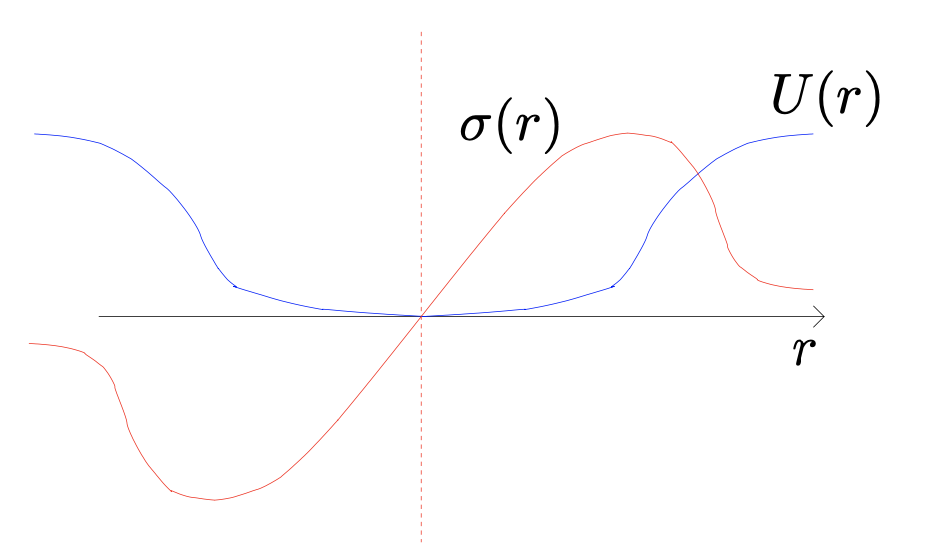
\includegraphics[scale=0.3]{qm11.png}
\end{center}

\subsection{Spherically symmetric potential well}\ \vspace{-1.5em}
\begin{example}
	Consider the potential well given by
\[
	U(r) = \begin{cases}
		0   & r \leq a \\
		U_0 & r > a
	\end{cases}
\]
where \( a, U_0 > 0 \).
The time-independent Schr\"odinger equation is
\[
	-\frac{\hbar^2}{2m} \sigma''(r) + U(r) \sigma(r) = E \sigma(r)
\]
\end{example}
We search for odd-parity bound states, \( 0 \le E \le U_0 \).
Let
\[
	k = \sqrt{\frac{2mE}{\hbar^2}};\quad \overline k = \sqrt{\frac{2m(U_0 - E)}{\hbar^2}}
\]
The solution for \( \sigma \) is
\[
	\sigma(r) = \begin{cases}
		A \sin(kr)           & r \leq a \\
		B e^{-\overline k r} & r > a
	\end{cases}
\]
The continuity condition at \( r = a \) can be imposed to find \( A \sin ka = B e^{-\overline k a} \).
The continuity of the derivative gives \( kA \cos ka = -\overline k B e^{-\overline k a} \).
Therefore,
\[
	-k \cot(ka) = \overline k;\quad k^2 + \overline k^2 = \frac{2mU_0}{\hbar^2}
\]
by rescaling
\[
	-\xi \cot \xi = \eta; \quad \xi^2 + \eta^2 = r_0^2
\]
where \( \xi = ka \) and \( \eta = \overline k a \), and \( r_0 = a\sqrt{2mU_0/\hbar} \).
\begin{center}
	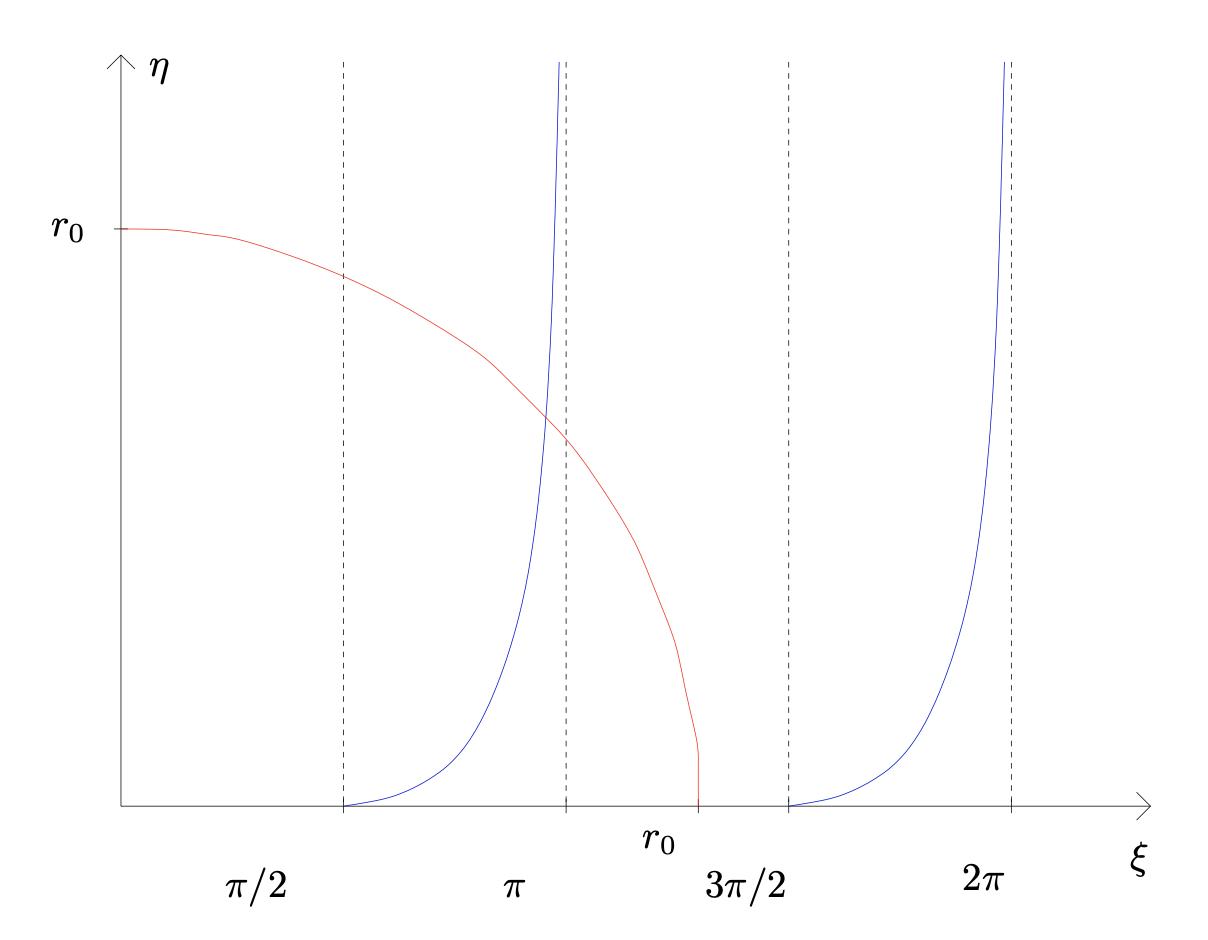
\includegraphics[scale=0.22]{qm12.png}
\end{center}
If \( r_0 < \frac{\pi}{2} \), we have no solutions because \( \xi \geq 0 \).
Equivalently, there are no solutions if
\[
	U_0 < \frac{\pi^2 \hbar^2}{8ma^2}
\]
There are two differences between the solution in 1D: 
\begin{enumerate}
	\item Below a given threshold for $U_0$, there does not exist any bound state in 3D, unlike one-dimensional case where we always find at least one bound state. 
	\item The solution 
	\[
		\chi(r) = \begin{cases}
			A \sin(kr)/r           & r \leq a \\
			B e^{-\overline k r}/r & r > a
		\end{cases}
	\]
	is bounded above by $ 1/r $ (up to a constant multiplication). 
\end{enumerate}

\section{Angular momentum in QM}
\subsection{Definition of angular momentum}
Recall that classically the angular momentum \( \bfL \) is given by
\[
	\bfL = \bfx \times \bfp
\]
Spherically symmetric potentials conserve classical angular momentum:
\[
	\dv{\bfL}{t} = \dot \bfx \times \bfp + \bfx \times \dot \bfp = 0
\]
Solving classical problems in this way allows us to reduce a three-dimensional problem into a two-dimensional problem, by considering motion on the plane \( \bfL \cdot \bfx = 0 \).
Then we reduce to one dimension by considering \( \hat \bfe_r \).
In quantum mechanics, we can do an analogous simplification.

\begin{definition}
	In Quantum Mechanics, the orbital angular momentum is an observable which corresponds to the operator,
	\[
	\begin{aligned}
	\hat{\mathbf{L}} &=\hat{\mathbf{x}} \times \hat{\mathbf{p}} \\
	&=-i \hbar \mathbf{x} \times \nabla
	\end{aligned}
	\]
	In index notation for Cartesian coordinates $\mathbf{x}=\left(x_1, x_2, x_3\right)$
	\[
	\hat{L}_i=\varepsilon_{i j k} \hat{x}_j \hat{p}_k=-i \hbar \varepsilon_{i j k} x_j \frac{\partial}{\partial x_k}
	\]
	where $\varepsilon_{i j k}$ is the Levi-Civita alternating tensor. Explicitly,
	\[
	\hat{\mathbf{L}}=-i \hbar\left(x_2 \frac{\partial}{\partial x_3}-x_3 \frac{\partial}{\partial x_2}, x_3 \frac{\partial}{\partial x_1}-x_1 \frac{\partial}{\partial x_3}, x_1 \frac{\partial}{\partial x_2}-x_2 \frac{\partial}{\partial x_1}\right)
	\]
\end{definition}

The difference between 1D and 3D are given as follows. 
\begin{center}
	\begin{tabular}{cc}
		\toprule 
		\textbf{1D} & \textbf{3D} \\ \midrule 
		$\displaystyle \pdv[2]{}{x}$  &  $\displaystyle \laplacian = \pdv[2]{}{x_1} + \pdv[2]{}{x_2} + \pdv[2]{}{x_3}$ \\[1em]
		$\displaystyle \hat p = -i \hbar \pdv{}{x}$ & $\displaystyle \hat{\mathbf{p}} = - i \hbar \grad = -i \hbar \left( \pdv{}{x_1},\pdv{}{x_2},\pdv{}{x_3} \right)$  \\ 
		$\displaystyle \hat{p}^2 = - \hbar^2 \pdv[2]{}{x}$ & $\displaystyle |\hat{\mathbf{p}}|^2 = - \hbar^2 \laplacian$\\ \bottomrule
	\end{tabular}
\end{center}

\subsection{Properties of angular momentum}

\begin{enumerate}
	\item The operators $\hat{L}_i$ are Hermitian, as all operators associated to physical observables.
	\item The different components of the angular momentum operator do not commute with each other: $\left[\hat{L}_i, \hat{L}_j\right] \neq 0$ for $i \neq j$. Thus, different components of angular momentum cannot be measured simultaneously.
	We can check this explicitly by computing the commutator,
	\[
	\begin{aligned}
	\left[\hat{L}_1, \hat{L}_2\right] &f\left(x_1, x_2, x_3\right)\\ 
	=\,&-\hbar^2\left[\left(x_2 \frac{\partial}{\partial x_3}-x_3 \frac{\partial}{\partial x_2}\right)\left(x_3 \frac{\partial}{\partial x_1}-x_1 \frac{\partial}{\partial x_3}\right)\right.\\ 
	&\left.-\left(x_3 \frac{\partial}{\partial x_1}-x_1 \frac{\partial}{\partial x_3}\right)\left(x_2 \frac{\partial}{\partial x_3}-x_3 \frac{\partial}{\partial x_2}\right)\right] f\left(x_1, x_2, x_3\right)
	\end{aligned}
	\]
	In the above equation many term cancels leaving,
	\[
	\begin{aligned}
	{\left[\hat{L}_1, \hat{L}_2\right] f } &=-\hbar^2\left(x_2 \frac{\partial}{\partial x_1}-x_1 \frac{\partial}{\partial x_2}\right) f\left(x_1, x_2, x_3\right) \\
	&=i \hbar \hat{L}_3 f\left(x_1, x_2, x_3\right)
	\end{aligned}
	\]
	A similar calculation for the other components confirms the commutation relations,
	\[
	\left[\hat{L}_2, \hat{L}_3\right]=i \hbar \hat{L}_1 \quad \text { and } \quad\left[\hat{L}_1, \hat{L}_3\right]=-i \hbar \hat{L}_2
	\]
	\item $\left[\hat{L}_i, \hat{L}_j\right]=i \hbar \varepsilon_{i j k} \hat{L}_k$, which combines the three independent commutation relations that we found above, using index notation.
\end{enumerate}

\subsection{Total angular momentum}

In Classical Mechanics the magnitude of the angular momentum is $L=|\mathbf{L}|$. Thus,
\[
L^2=L_1^2+L_2^2+L_3^2
\]
\begin{definition}
	In Quantum Mechanics we define the total angular momentum operator,
	\[
	\hat{L}^2=\hat{L}_1^2+\hat{L}_2^2+\hat{L}_3^2
	\]
\end{definition}

\subsection{Properties of total angular momentum}
For proofs, see Dr Ubiali's notes. 
\begin{enumerate}
	\item The total angular momentum $\hat{L}^2$ commutes with each of the components of angular momentum $\hat{L}_i, i=1,2,3$
	\item The total angular momentum operator commutes with an Hamiltonian featuring a spherically symmetric potential, i.e. 
	\[
		\qty[\hat H, \hat L^2] = \qty[\hat H, \hat L_i] = 0. 
	\]
	This means that the angular momentum operators care nothing for how the wavefunctions depend on the radial coordinate $r$. The angular momentum of a state is, perhaps unsurprisingly, encoded in how the wavefunction varies in the angular directions $\theta$ and $\Phi$.
\end{enumerate}

\subsection{Commutativity of angular momentum operators}
The set \( \qty{ \hat H, \hat L^2, \hat L_i } \) commutes pairwise.
By convention, we choose \( i = 3 \) to extract the \( z \) component of the angular momentum.
Hence,
\begin{enumerate}
	\item We can find joint eigenstates of the three operators, and such eigenstates can be chosen to form a basis for the Hilbert space \( \mathcal H \).
	\item The corresponding eigenvalues \( \abs{L}, L_z, E \) can be measured simultaneously to an arbitrary precision.
	\item The set of operators is maximal, in other words, we cannot construct another independent operator (other than the unit operator) which commutes with each of $\hat{H}, \hat{L}^2$ and $\hat{L}_3$.
\end{enumerate}

\subsection{Joint eigenfunctions of anglar momentum}
To find joint eigenfunctions of $ \hat{L}^2 $ and $ \hat{L}_3 $, write $ \hat{\mathbf{L}} $ in spherical coordinates (see Appendix A.7 of Dr Ubiali's notes): 
\[
	\begin{aligned}
		\hat{L}^2 &=-\frac{\hbar^2}{\sin ^2(\theta)}\left[\sin (\theta) \frac{\partial}{\partial \theta}\left(\sin (\theta) \frac{\partial}{\partial \theta}\right)+\frac{\partial^2}{\partial \phi^2}\right] \\
		\hat{L}_3 &=-i \hbar \frac{\partial}{\partial \phi}
	\end{aligned}
\]
Now we search for eigenfunctions of these operators.
\[
	\hat L^2 Y(\theta, \phi) = \lambda Y(\theta, \phi);\quad \hat L_3 Y(\theta, \phi) = \hbar m Y(\theta, \phi)
\]
Consider the eigenvalue equation for $ \hat L_3 $
\[
	- i \hbar \pdv{}{\phi} Y(\theta,\phi) = \hbar m Y(\theta,\phi)
\] 
We find solutions of the form $ Y(\theta,\phi) = y(\theta) x(\phi) $. Note that plugging in back we find
\[
	-i\hbar y(\theta) x'(\phi) = \hbar m y(\theta) x(\phi)
\]
Hence \( y(\theta) \) is arbitrary, and further
\[
	-i\hbar x'(\phi) = \hbar m x(\phi) \implies x(\phi) = e^{i m \phi}
\]
But wavefunctions must be single-valued functions on $\mathbb{R}^3$ and should therefore be invariant under $\phi \rightarrow \phi+2 \pi$. The function $\exp (i m \phi)$ is invariant provided,
\[
\exp (2 \pi i m)=1  \implies  m \in \mathbb{Z}. 
\]
Thus the eigenvalues of $\hat{L}_3$ have the form $\hbar m$ for integer $m$. Equivalently, the $z$-component of angular momentum is \textit{quantised} in integer multiples of $\hbar$. This agrees with Bohr's quantisation condition.
Similarly we must have,
\[
\hat{L}^2 y(\theta) \exp (i m \phi)=\lambda y(\theta) \exp (i m \phi)
\]
for some eigenvalue $\lambda$. Using the explicit form for $\hat{L}^2$ we find that $y(\theta)$ must obey the equation,
\[
\frac{1}{\sin (\theta)} \frac{\partial}{\partial \theta}\left(\sin (\theta) \frac{\partial y(\theta)}{\partial \theta}\right)-\frac{m^2}{\sin ^2(\theta)} y(\theta)=-\frac{\lambda}{\hbar^2} Y(\theta)
\]

This is the associate Legendre equation.
The solutions of \( y(\theta) \) are the associate Legendre functions.
\[
	y(\theta) = P_{\ell,m}(\cos \theta) = (\sin \theta)^{\abs{m}} \dv[\abs{m}]{(\cos \theta)}  P_\ell(\cos \theta)
\]
where the \( P_\ell \) are the Legendre polynomials.
Since the ordinary Legendre polynomials are of degree \( \ell \), we must have \( \abs{m} \leq \ell \) to obtain a nonzero solution.
This corresponds to the classical notion that \( \abs{L_z} \leq \abs{L} \) for a physical solution.
The eigenvalues of \( \hat L^2 \) are
\[
	\lambda = \ell(\ell+1) \hbar^2
\]
with \( \ell \in \qty{0, 1, 2, \dots} \).
Thus,
\[
	Y_{\ell, m}(\theta, \phi) = P_{\ell,m}(\cos\theta) e^{im\phi}
\]
The \( Y \) functions are called the \textbf{spherical harmonics}.
The parameters \( \ell, m \) are known as the \textbf{quantum numbers} of the eigenfunction; \( \ell \) is the \textbf{total angular momentum} quantum number and \( m \) is the \textbf{azimuthal} quantum number.

The constraint $-\ell \leq m \leq \ell$ is the quantum version of the classical inequality,
\[
-|\mathbf{L}| \leq L_z \leq+|\mathbf{L}|
\]
which follows because $L_z=|\mathbf{L}| \cos (\theta)$.

Examples of normalised eigenfunctions are
\begin{align*}
	Y_{0,0}     & = \frac{1}{\sqrt{4 \pi}}                             \\
	Y_{1,0}     & = \sqrt{\frac{3}{4 \pi}} \cos \theta                 \\
	Y_{1,\pm 1} & = \mp \sqrt{\frac{3}{8 \pi}} \sin \theta e^{-i \phi}
\end{align*}
All spherical harmonics can be shown to be orthornormal:
\[
	\int_0^{2 \pi} \dd \phi \int_{-1}^{+1} \dd \cos \theta\; Y_{l^{\prime}, m^{\prime}}^*(\theta, \phi) Y_{l, m}(\theta, \phi)=\delta_{l l^{\prime}} \delta_{m m^{\prime}}
\]

\section{The hydrogen atom}
We now apply the above to solve the hydrogen atom. 
\begin{definition}
	The hydrogen $(\mathrm{H})$ atom consists of a single proton $p^{+}$and an electron $e^{-}$.
\end{definition}

As before treat the proton as stationary at the origin of spherical polar coordinates, i.e. we model the hydrogen atom by treating the proton as infinitely massive and at rest at the origin. The Coulomb attraction,
\[
F(r)=-\frac{\partial U(r)}{\partial r}=-\frac{e^2}{4 \pi \varepsilon_0 r^2}
\]
corresponds to a potential
\[
U(r)=-\frac{e^2}{4 \pi \varepsilon_0 r}.
\]
The time-independent Schr\"odinger equation for the hydrogen atom is
\[
	-\frac{\hbar^2}{2m_e} \laplacian{\chi(r, \theta, \phi)} - \frac{e^2}{4 \pi \varepsilon_0} \frac{1}{r} \chi(r, \theta, \phi) = E \chi(r,\theta, \phi)
\]
Writing the Laplacian in spherical polar coordinates,
\[
	\laplacian{} = \frac{1}{r} \pdv[2]{r} + \frac{1}{r^2 \sin^2 \theta} \qty( \sin \theta \pdv{\theta} \sin \theta \pdv{\theta} + \pdv[2]{\phi} )
\]
Hence,
\[
	\hat L^2 = \frac{\hbar^2}{\sin^2\theta} \qty[ \sin \theta \pdv{\theta} \sin \theta \pdv{\theta} + \pdv[2]{\phi} ] \implies -\hbar^2 \laplacian{} = -\frac{\hbar^2}{r} \pdv[2]{r} r + \frac{\hat L^2}{r^2}
\]
Thus we can rewrite the TISE as
\[
	-\frac{\hbar^2}{2m_e} \frac{1}{r} \qty( \pdv[2]{r} \qty(r \chi) ) + \frac{\hat L^2}{2 m_e r^2} \chi - \frac{e^2}{4 \pi \varepsilon_0 r} \chi = E \chi
\]
Because eigenfunctions of $ \hat H $ are also eigenfunctions of $ \hat L^2, \hat L_3 $, we now look for a simultaneous eigenstate of
\[
\left\{\hat{H}, \hat{L}^2, \hat{L}_3\right\}
\]
by setting
\[
\chi(r, \theta, \phi)=R(r) Y_{l, m}(\theta, \phi)
\]
where $Y_{l, m}$ is a spherical harmonic.

Since \( \chi \) is an eigenfunction of \( \hat L^2 \),
\[
	\hat L^2 (R(r) Y_{\ell,m}(\theta,\phi)) = R(r) \hbar^2 \ell (\ell+1)Y_{\ell,m}(\theta, \phi)
\]
Substituting into the TISE,
\begin{align*}
	&-\frac{\hbar^2}{2m_e} \qty( \pdv[2]{R}{r} 
	+ \frac{2}{r} \pdv{R}{r} ) Y_{\ell,m}(\theta, \phi) \\ 
	&+ \frac{\hbar^2}{2 m_e r^2} \ell(\ell+1) R(r)Y_{\ell,m}(\theta, \phi) \\ 
	&-\frac{e^2}{4 \pi \varepsilon_0 r} R(r)Y_{\ell,m}(\theta,\phi) = E R(r)Y_{\ell,m}(\theta,\phi)
\end{align*}
Cancelling the spherical harmonic, we end up with an 1D equation for the radial part:
\[
	-\frac{\hbar^2}{2m_e} \qty( \dv[2]{R}{r} + \frac{2}{r} \dv{R}{r} ) + \underbrace{\qty(\frac{\hbar^2}{2 m_e r^2} \ell(\ell+1) - \frac{e^2}{4 \pi \varepsilon_0 r})}_{U_{\mathrm{eff}} = \text{ effective potential}} R(r) = E R(r)
\]
\subsection{The radial wavefunction $ \ell=0 $}

When $ \ell=0 $, $ U_{\text{eff}} = U_{\text{Coulomb}} $, and by grouping quantaties up
\[
	\nu^2 = - \frac{2m E}{\hbar^2} \quad \beta = \frac{e^2m}{2\pi\epsilon_0 \hbar^2}
\]
we get
\[
	R'' + \frac{2}{r} R' + \qty(\frac{\beta}{r} - \nu^2 )R = 0
\]
We have 2 observations:
\begin{enumerate}
	\item The asymptotic behaviour as $ r\to \infty $ is determined by 
	\[
		R'' - \nu^2 R = 0 \iff R(r) \sim e^{\pm r \nu}
	\]
	Take $ R(r) = e^{-r\nu} $ for normalisation condition. 
	\item At $r=0$, $R$ must be finite. 
\end{enumerate}

As in the analysis of the harmonic oscillator, it is convenient to separate out the exponential dependence of the eigenfunction and look for a solution of the form,
\[
R(r)=f(r) \exp (-\nu r) .
\]
If we plug it into the Schrödinger equation, it becomes
\[
\frac{\rmd^2 f}{\rmd r^2}+\frac{2}{r}(1-\nu r) \frac{\rmd f}{\rmd r}+\frac{1}{r}(\beta-2 \nu) f=0
\]
It is homogeneous and linear with $r=0$ as a regular point, so we can use series method:
\[
	f(r)=r^c \sum_{n=0}^{\infty} a_n r^n
\]
Substituting back we get 
\[
	\sum_{n=0}^{\infty}\left[a_n(c+n)(c+n-1) r^{c+n-2}+\frac{2}{r}(1-\nu r) a_n(c+n) r^{c+n-1}+(\beta-2 \nu) a_n r^{c+n-1}\right]=0
\]
The lowest power of $r$ which occurs on the LHS is $a_0 r^{c-2}$ with coefficient $c(c-1)+2 c=$ $c(c+1)$. Equating this to zero yields the indicial equation
\[
c(c+1)=0
\]
with roots $c=0$ and $c=-1$. However, the root ${c}=-1$ would imply $\chi(r) \sim 1 / r$ near $r=0$. This yields a singular eigenfunction which violates the boundary condition at the origin. Thus we choose root $c=0$ and our series solution simplifies to
\[
f(r)=\sum_{n=0}^{\infty} a_n r^n
\]
If we now collect all terms of order $r^{n-2}$ on the LHS and equate them to zero to get
\[
n(n-1) a_n+2 n a_n-2 \nu(n-1) a_{n-1}+(\beta-2 \nu) a_{n-1}=0
\]
or more simply
\[
a_n=\frac{(2 \nu n-\beta)}{n(n+1)} a_{n-1}
\]
The above recurrence relation determines all the coefficients $a_n$ in the series in terms of the first coefficent $a_0$. As in our analysis of the harmonic oscillator, there are two possibilities,
\begin{itemize}
	\item The series terminates. In other words $\exists N>0$ such that $a_n=0 \forall n \geq N$.
	\item The series does not terminate. In other words $\nexists N>0$ such that $a_n=0 \forall$ $n \geq N$
\end{itemize}
\begin{proposition}
	If the series does not terminate, then the function $ \chi(r) = f(r) e^{-\nu r} $ is not normalisable.
\end{proposition}
See Prof Ubiali's notes. 

Hence \( g \) must be a polynomial with first zero coefficient \( a_{n_{\max}} \).
Here,
\[
	2\nu(n_{\max} + \ell) - \beta = 0
\]
We define \( N = n_{\max} + \ell \), so \( 2 \nu N - \beta = 0 \) giving \( \nu = \frac{\beta}{2N} \).
Note that \( N > \ell \) since \( n_{\max} > 0 \).
We can then find the energy level to be
\[
	E_N = -\frac{e^4 m_e}{32 \pi^2 \varepsilon_0^2 \hbar^2} \frac{1}{n^2}
\]
which is an identical energy spectrum as we found before when not considering angular momentum (using the Bohr model).
For each \( E_N \), we have \( N = n_{\max} + \ell \) so there can be \( \ell = 0, \dots, N-1 \) and \( m = -\ell, \dots, \ell \).
Hence, the degeneracy of the solution for each \( N \) is
\[
	D(N) = \sum_{\ell=0}^{N-1} \sum_{m=-\ell}^\ell 1 = N^2
\]
So the degeneracy increases quadratically with the energy level.
For example, for \( N = 2 \) there are four possible eigenfunctions with the same energy.
The eigenfunctions are now dictated by three quantum numbers.
\[
	\chi_{N,\ell,m}(r,\theta,\phi) = R_{N,\ell}(r)Y_{\ell,m}(\theta,\phi) = r^\ell g_{N,\ell}(r) e^{-\frac{\beta r}{2N}} Y_{\ell,m}(\theta,\phi)
\]
where \( g_{N,\ell} \) is a polynomial of degree \( N - \ell - 1 \) defined by the recurrence relation
\[
	a_k = \frac{2\nu}{k} \frac{k + \ell - N}{k + 2\ell + 1} a_{n-1}
\]
These are the generalised Laguerre polynomials, often written
\[
	g_{N,\ell}(r) = L_{N - \ell - 1}^{2\ell + 1}(2r)
\]
The quantum number \( N \in \qty{0, 1, \dots} \) is known as the \textit{principal} quantum number.

\subsection{Comparison to Bohr model}
In the Bohr model, the energy levels were predicted accurately.
Further, the maximum of the radial probability corresponds to the orbits found in the Bohr model:
\[
	\dv{r} \qty( \abs{\chi_{N,0,0}(r)}^2 r^2) = 0
\]
The classical trajectory, and the assumption about the angular momentum \( L^2 = N^2 \hbar^2 \), were incorrect.
The angular momentum found in quantum mechanics is \( L^2 = \ell(\ell+1) \hbar^2 \), which corresponds closely with the Bohr model for large \( \ell \).

\subsection{Other elements of the periodic table}
The above solution does not hold for other elements of the periodic table.
Generalising to a nucleus with clarge \( +ze \) and \( z \) orbiting electrons, we could model this as
\[
	\chi(x_1, \dots, x_z) = \chi(x_1) \dots \chi(x_N);\quad E = \sum_{j=1}^N e_j
\]
This approximation can be acceptable for small \( z \), but diverges very quickly from the true solution as \( z \) increases, due to the electron-electron interactions and the Pauli exclusion principle.

\end{document}